\documentclass{jot}

\usepackage[utf8]{inputenc}
\usepackage[T1]{fontenc}
\usepackage{lmodern}
\usepackage[english]{babel}
\usepackage{microtype} % optional, for aesthetics
\usepackage{tabularx} % nice to have
\usepackage{booktabs} % necessary for style
\usepackage{graphicx}
\graphicspath{{./figures/}}
\usepackage{listings}
\usepackage{cite}
\usepackage{multirow}
\usepackage{hhline}
\usepackage{caption}
\usepackage{makecell}
\usepackage{ragged2e}
\usepackage{parskip}
\usepackage{wrapfig}
\usepackage{array}
\usepackage{float}
\usepackage[english]{babel}
\usepackage{lipsum}
\usepackage{subcaption}
\usepackage[linesnumbered,ruled]{algorithm2e}
\usepackage{courier}
\usepackage{hyperref}
\hypersetup{colorlinks=true,allcolors=blue}
\usepackage{listings}
\usepackage{float}
\lstset{
    basicstyle=\ttfamily,
    frame=none, 
    breaklines=true,
    numbers=left,
    xleftmargin=2.5em,
    framexleftmargin=0em,
    emphstyle=\textbf,
    float=t
}
\lstdefinestyle{ocl}{
    emph={
        context, inv
    }
}
\lstdefinestyle{cbp}{
    basicstyle=\ttfamily\scriptsize,
    emph={
        session, create, type,
        set, to, add, hire
    }
}
\lstdefinestyle{xmi}{
    basicstyle=\ttfamily\scriptsize,
    emph={
        Node, children
    }
}
\lstdefinestyle{xml}{
    basicstyle=\ttfamily\scriptsize,
    emph={
        register, create, add, to, resource, at,
        from, eattribute, remove, ereference,
        set, unset, session, Roy, Jen,
        Moss, Richmond
    }
}
\lstdefinestyle{java}{
    basicstyle=\ttfamily\scriptsize,
    emph={
        case, $unset$,
        instanceof, else, if, void,
        new, UnsetEAttributeEvent,
        UnsetEReferenceEvent,
        @override, public, class, extends
    }
}
\lstdefinestyle{eol}{
    basicstyle=\ttfamily\scriptsize,
    emph={
        var, new, for, in, create, set, with, type, at,
        unset, to, add, remove, delete, register, move,
        from, position, from, move-within, session, \.
    }
}

% $ChangeHybridEventAdapter$

\hyphenation{op-tical net-works semi-conduc-tor Hybrid-Change-Event-Adapter Hybrid-XMI-Change-Event-Adapater
    Hybrid-Neo-EMF-Change-Event-Adapater change-Events Change-Event-Adapter EContent-Adapter notify-Changed Hybrid-Resource Resource-Impl state-Based-Resource cbp-Output-Stream Output-Stream Hybrid-Change-Event-Adapater Output-Stream Hybrid-XMI-Resource-Impl Hybrid-Neo-EMF-Resource-Impl Persistence-Resource change-Events
}

\definecolor{gray1}{gray}{0.90}
\definecolor{gray2}{gray}{0.95}

%%% Article metadata
\title{Harnessing Change-based Persistence to Optimise Model Comparison}
\runningtitle{Harnessing Change-based Persistence to Optimise Model Comparison}

\author[affiliation={york,kalbis}, nowrap, photo=avatar]
    {Alfa Yohannis}
    {is a PhD Student in the Department of Computer Science at the University of York, United Kingdom (\email{alfa.yohannis@merahputih.id}).}
\author[affiliation=york, nowrap, photo=avatar]
{Horacio Hoyos Rodriguez}
{is a Research Staff in the Department of Computer Science at the University of York, United Kingdom (\email{horacio\_hoyos\_rodriguez@ieee.org}).}
\author[affiliation=keele, nowrap, photo=avatar]
{Fiona Polack}
{is a Professor of Software Engineering in the School of Computing and Maths at the Keele University, United Kingdom  (\email{f.a.c.polack@keele.ac.uk}).}
\author[affiliation=york, nowrap, photo=avatar]
{Dimitris Kolovos}
{is a Professor of Software Engineering in the Department of Computer Science at the University of York, United Kingdom (\email{dimitris.kolovos@york.ac.uk}).}

\affiliation{york}{Department of Computer Science, University of York, United Kingdom}
\affiliation{keele}{School of Computing and Maths, Keele University, United Kingdom}
\affiliation{kalbis}{Department of Computer Science, Kalbis Institute, Indonesia}

\runningauthor{Alfa Yohannis, Horacio Hoyos Rodriguez, Fiona Polack, Dimitris Kolovos}

\jotdetails{
    volume=V,
    number=N,
    articleno=M,
    year=2011,
    doisuffix=jot.201Y.VV.N.aN,
    license=ccbynd % choose from ccby, ccbynd, ccbyncnd
}


\begin{document}
\renewcommand{\thelstlisting}{\arabic{lstlisting}}
\renewcommand{\labelitemi}{$\bullet$}
\newcommand{\dk}[1]{\textbf{[DK: #1]}}
\newcommand{\And}{\textnormal{\textbf{and }}}
\newcommand{\Is}{\textnormal{\textbf{is }}}
\newcommand{\Not}{\textnormal{\textbf{not }}}
\newcommand{\In}{\textnormal{\textbf{in }}}
\newcommand{\Or}{\textnormal{\textbf{or }}}

\begin{abstract}
Comparison of two large models can be time-consuming since every element of a model has to be visited, matched, and compared with its respective element in the other model. This downside causes a bottleneck in collaborative modelling especially when identifying differences between two versions of a model is desirable. This paper harnesses change-based persistence to localise the comparison of models so that only elements affected by recent changes that are compared. This approach leads to a faster model differencing as opposed to the traditional state-based model comparison. 
\end{abstract}

\keywords{Model Comparison; Change-based Persistence; State-based Persistence.}

\vspace{-10pt}
\section{Introduction}
\label{sec:introduction}

\vspace{-5pt}

In modelling and model management, it is common to find that many versions or variants of models exist. These models are commonly persisted in their snapshots, in their state-based format, which capture the states of models at the time they were taken. Traditional model comparison activities can be applied to these models to highlight their variations. However, comparing large models in state-based format can be lengthy since every element of each model has to be visited, matched to an element in other models, and compared to identify their differences. This lengthy comparison can slow down the construction of large models, particularly in a collaborative modelling setting. 

In our previous work \cite{DBLP:conf/models/YohannisKP17,yohannis2018towards,DBLP:conf/models/YohannisRPK18}, we have proposed a change-based persistence (CBP), an alternative approach to persist EMF models \cite{steinberg2008emf} in change-based format. Instead of persisting models in their final states, the approach persists models in their complete history of changes. We also argued that the incremental, detailed information contained in CBP could be exploited to support model comparison, incremental model transformation, and model analytics.

In this paper, we present our approach in harnessing CBP to achieve faster model comparison in the context of EMF. The nature of CBP that records recent changes with detailed information facilitates the identification of elements that have been modified since the previous persisted version. The availability of this information eliminates the necessity to visit, match, and diff every element of models being compared. Thus, we can localise model comparison only to recently affected elements which in turns can reduce the time used for model comparison.

This paper is structured as follows. Section \ref{sec:change-based_persistence} introduces the concept of change-based persistence. Sections \ref{sec:model_comparison} overviews of the state-based approach to compare models. Section \ref{sec:change_based_approach_for_comparing_models} presents our change-based approach to speed up model comparison and its implementation. Section \ref{sec:evaluation} presents our experimental results and evaluation. Section \ref{sec:related_work} provides an overview of related work, and Section \ref{sec:conclusion_and_future_work} concludes with a discussion on directions for future work.

\vspace{-10pt}
\section{Change-based Persistence}
\label{sec:change-based_persistence}

\vspace{-5pt}
Change-based persistence is an alternative approach to state-based persistence (SBP) of models. Instead of persisting the last state of a model, CBP persists the overall history of changes of a model \cite{yohannis2018towards}. For example, in SBP approach, when we save the UML class diagram in Fig. \ref{fig:origin} in standard XMI format, we only obtain the last state of the model as the List. \ref{lst:originxmi} shows. In contrast, when we develop the model in CBP approach, a system captures all the changes of the model and persists them into a CBP file as shown in List. \ref{lst:origincbp}\footnote{In implementation, the CBP is persisted in XML-like format, not in pseudo-format.}. The file consists of events generated by changes. Each change event contains information about the type of the operation applied as well the as values, elements, or features involved. Replaying the change events in List. \ref{lst:origincbp} produces the eventual model as in Fig. \ref{fig:origin}.

\vspace{-20pt}
\begin{minipage}[t]{0.59\linewidth} 
    \centering
    \begin{lstlisting}[style=eol,caption={The simplified XMI of the model in Fig. \ref{fig:origin}.},label=lst:originxmi]
    <uml:Class id="x" name="Math">
    <operation id="a" name="abs"/>
    <operation id="b" name="mean"/>
    <operation id="c" name="pow"/>
    </uml:Class>
    \end{lstlisting}
    \vspace{-25pt}
    \begin{figure}[H]
        \centering    
        \hfill
        \begin{subfigure}[t]{0.2\linewidth}
            \centering
            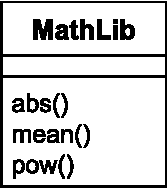
\includegraphics[width=\linewidth]{OriginalClassDiagram}
            \caption{origin}
            \label{fig:origin}
        \end{subfigure}
        \hfill
        \begin{subfigure}[t]{0.2\linewidth}
            \centering
            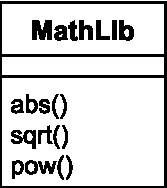
\includegraphics[width=\linewidth]{LeftClassDiagram}
            \caption{left}
            \label{fig:left}
        \end{subfigure}
        \hfill
        \begin{subfigure}[t]{0.2\linewidth}
            \centering
            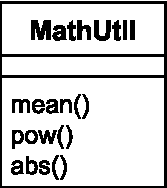
\includegraphics[width=\linewidth]{RightClassDiagram}
            \caption{right}
            \label{fig:right}
        \end{subfigure}
        \hfill
        \label{fig:versions}
        \caption{Different versions of a model.}
    \end{figure}
\end{minipage}
\hfill
\begin{minipage}[t]{0.39\linewidth}
    \begin{lstlisting}[style=eol,caption={The pseudo-formatted CBP of the model in Fig. \ref{fig:origin}.},label=lst:origincbp]
    session "origin"
    create x type Class
    set x.name to "Math" 
    create a type Operation
    set a.name to "abs" 
    create b type Operation
    set b.name to "mean" 
    create c type Operation
    set c.name to "pow" 
    add a to x.operations at 0
    add b to x.operations at 1
    add c to x.operations at 2
    \end{lstlisting}
\end{minipage}

\vspace{-5pt}
\section{State-based Model Comparison}
\label{sec:model_comparison}

\vspace{-5pt}
In a collaborative modelling setting, a model is commonly developed in parallel -- thus produces different versions. Let's say that the model in Fig. \ref{fig:origin} is modified by two different modellers in parallel. The first modeller produces the model in Fig. \ref{fig:left} (the left model), and the second one yields the model in Fig. \ref{fig:right} (the right model) producing XMI files as shown in List. \ref{lst:leftxmi} and List. \ref{lst:rightxmi} respectively.

At some point, we want to compare these two models in order to identify their differences for analytics or conflicts when merging. The common approach to compare models is to create matches between the elements of both models and diff them \cite{DBLP:conf/sfm/BroschKLSWW12,emfcompare2018developer}. Generally, the matching process iterates through all the elements of the models being compared and matches them by their identifiers or through a similarity mechanism if they have none \cite{DBLP:conf/sfm/BroschKLSWW12,emfcompare2018developer}. After that, the diffing process then starts finding differences between the matched elements and all their features commonly using the Longest Common Subsequence (LCS) algorithms, e.g. \cite{DBLP:journals/algorithmica/Meyers86}. 

\vspace{-10pt}
\begin{minipage}[t]{0.49\linewidth} 
    \begin{lstlisting}[style=eol,caption={The simplified XMI of the left model in Fig. \ref{fig:left}.},label=lst:leftxmi]
    <uml:Class id="x" name="MathLib">
    <operation id="a" name="abs/>
    <operation id="d" name="sqrt"/>
    <operation id="c" name="pow"/>
    </uml:Class>
    \end{lstlisting}
\end{minipage}
\hfill
\begin{minipage}[t]{0.49\linewidth}
    \begin{lstlisting}[style=eol,caption={The simplified XMI of the right model in Fig. \ref{fig:right}.},label=lst:rightxmi]
    <uml:Class id="x" name="MathUtil">
    <operation id="b" name="mean"/>
    <operation id="c" name="pow"/>
    <operation id="a" name="abs"/>
    </uml:Class>
    \end{lstlisting}
\end{minipage}

In our example, the matching iterates through all the elements of both model using their identifiers. The matching process yields 3 matches, $m_1$ = (\textsf{x}, \textsf{x}), $m_2$ = (\textsf{a}, \textsf{a}), and $m_3$ = (\textsf{c}, \textsf{c}), and 2 unmatched elements, $um_1$ = (\textsf{d},) and $um_2$ = (, \textsf{b}). The diffing process then iterates through all the matches and unmatches. Using the LCS algorithm, in the first match, it identifies that both elements \textsf{x} are different in their \textsf{name} and \textsf{operations} features. 
The left \textsf{x}'s \textsf{name} is ``MathLib'' while the other \textsf{x}'s \textsf{name} is ``MathUtil'' (diff $d_1$). The \textsf{operations} features are different in their contents -- the left \textsf{operations} feature does not contain elements \textsf{b} (diff $d_2$), the left \textsf{operations} feature contains element \textsf{d} 
that does not exist in the right \textsf{operations} (diff $d_3$), and the positions of element \textsf{c} that are different in both features (diff $d_4$).

Similar to EMF Compare \cite{emfcompare2018developer}, this paper views a left model as a reference model, which means that differences are expressed as changes applied to a right model so that it equals to a reference model -- a left model. To express differences, we used the following elements: \textsf{LeftContainer}, \textsf{RightContainer}, \textsf{LeftFeature}, \textsf{RightFeature} \textsf{LeftPosition}, \textsf{RightPosition}, \textsf{LeftValue}, \textsf{RightValue}, and \textsf{Kind}. The \textit{*Container}, \textit{*Feature}, and \textit{*Value} are the target element, feature, and value involved in a difference. \textsf{*Position} is the position of a value in a feature. \textit{Kind} is the type of difference. It can be one of these types: \textsf{CHANGE}, \textsf{ADD}, \textsf{DELETE}, and \textsf{MOVE}. \textsf{CHANGE} means a pair of features -- single-valued attributes or non-containment references -- are different in their values. \textsf{ADD} indicates that a value does not exist in the right model thus it requires the addition of the value. \textsf{DELETE} is the counterpart of \textsf{ADD}. \textsf{MOVE} indicates that matched elements are different in their locations, whether they are in the same features or cross features. 

Based on these definitions, we formalise the identified previously as $ds_{n}$ = [$LeftContainer_n$, $RightContainer_n$, $LeftFeature_n$, $RightFeature_n$, $LeftPosition_n$, $RightPosition_n$, $LeftValue_n$, $RightValue_n$, $Kind_n$]. Thus, $ds_{1}$ =  [\textsf{x}, \textsf{x}, \textsf{name}, \textsf{name}, 0, 0, ``MathLib'', ``Mathutil'', \textsf{CHANGE}], $ds_{2}$ = [\textsf{x}, \textsf{x}, \textsf{operations}, \textsf{operations}, ?, 0, ?, \textsf{b}, \textsf{DELETE}], $ds_{3}$ = [\textsf{x}, \textsf{x}, \textsf{operations}, \textsf{operations}, 1, ?, \textsf{d}, ?, \textsf{ADD}], and $ds_{4}$ = [\textsf{x}, \textsf{x}, \textsf{operations}, \textsf{operations}, 2, 1, \textsf{c}, \textsf{c}, \textsf{MOVE}]. Fig. \ref{fig:xmi_comparison} depicts the mapping of these diffs on the left and right models. Applying these diffs as changes to the right model will transform it into the left model.  

\vspace{-20pt}
\begin{figure}
    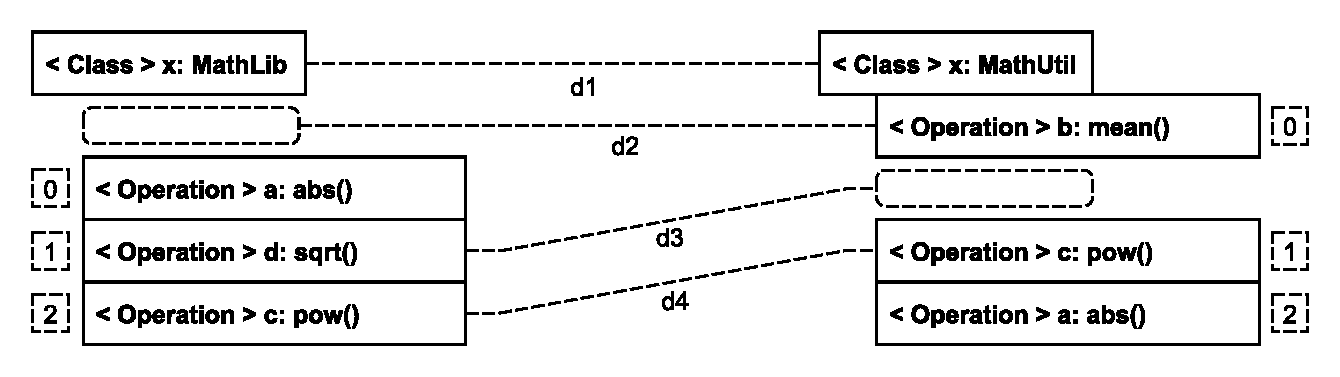
\includegraphics[width=\linewidth]{XmiComparison}
    \caption{A model comparison of the left and right models in Listings \ref{lst:leftxmi} and \ref{lst:rightxmi}.}
    \label{fig:xmi_comparison}
\end{figure}

\vspace{-20pt}
\section{Change-based Approach for Comparing Models}
\label{sec:change_based_approach_for_comparing_models}

\vspace{-20pt}
\begin{figure}
    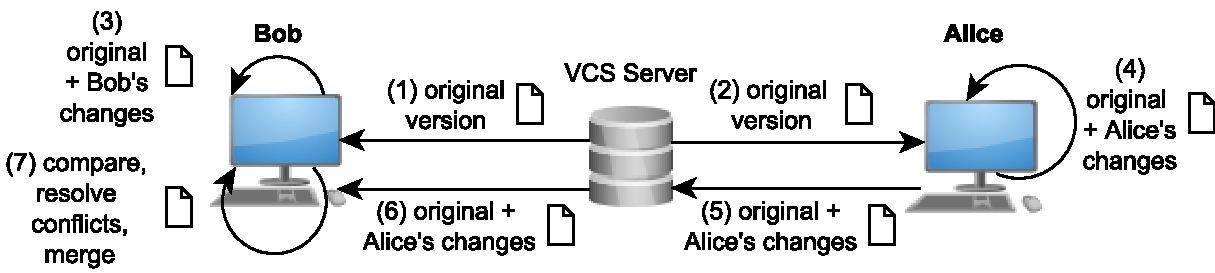
\includegraphics[width=\linewidth]{VCS}
    \caption{A case of the use of CBP in a collaborative modelling.}
    \label{fig:vcs}
\end{figure}

\vspace{-10pt}
In the context of collaborative modelling using CBP, let's say that the file of the CBP in \ref{lst:origincbp} already existed in a text-based Version Control System (VCS) server (Fig. \ref{fig:vcs}). Both modellers checkout the original CBP (steps 1 and 2) and modify it (steps 3 and 4). Changes made by the left and right modellers will be appended to the original CBP producing two different CBP representation as displayed in Listings \ref{lst:leftcbp} and \ref{lst:rightcbp}\footnote{Both CBPs only present the changes after the last line of the original version (start from line 19). In implementation, the changes are appended to the original version.} -- capturing different courses of modification made by the modellers. The right developer then commits her work (original + right version) to the VCS. Since there is no new commit on the VCS, the commit process is straightforward (step 5). The left developer then decides to also commit his work (original + left version) to the VCS, thus his machine downloads the current version from the server (step 6). However, since the original version has been updated since his last checkout, he has to perform a model comparison to check the differences, and possible conflicts, between his version (original + left version) and the updated original version (original + right version). 

\begin{minipage}[t]{0.49\linewidth}    
    \begin{lstlisting}[firstnumber=13,style=eol,caption={The CBP of the model in Fig. \ref{fig:left} (left version).},label=lst:leftcbp]
    session "left"
    set x.name from "Math" to "MathLib"
    create d type Operation
    set d.name to "sqrt"
    add d to x.operations at 1
    remove b in x.operations at 2
    delete b
    \end{lstlisting}
\end{minipage}
\hfill
\begin{minipage}[t]{0.49\linewidth}
    \begin{lstlisting}[firstnumber=13,style=eol,caption={The CBP of the model in Fig. \ref{fig:right} (right version).},label=lst:rightcbp]
    session "right"
    move a in x.operations from 0 to 2
    set x.name from "Math" to "MathUtil"
    \end{lstlisting}
\end{minipage}

Since both modellers work using CBP, we can exploit the persistence to improve the previous model comparison. For example, we do not need to visit, match, and differentiate both elements \textsf{c} in the running example as it is not affected by the recent changes in both CBPs; only the affected features by the recent changes to be compared -- not all features. 

In performing the comparison, our approach has three phases: event loading, element tree construction, and diff computation. These phases are represented as methods \textsf{loadEvents}, \textsf{contructElementTree}, and \textsf{computeDifferences} methods in class \textsf{CBPComparison} in Fig. \ref{fig:approach_class_diagram}. 

\vspace{-10pt}
\begin{figure}
    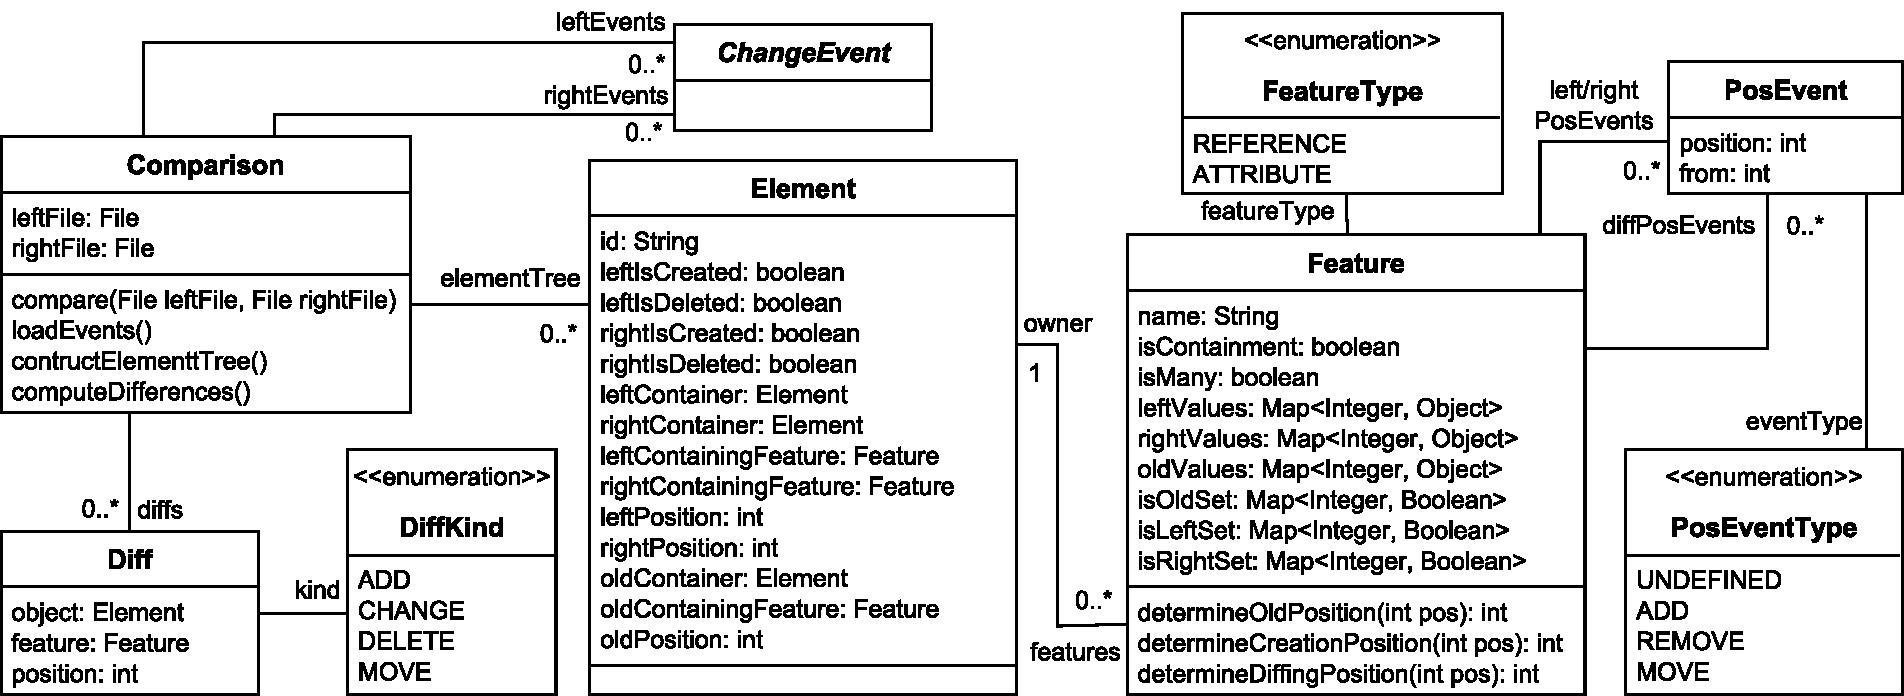
\includegraphics[width=\linewidth]{TreeClassDiagram}
    \caption{A class diagram showing the core components of the change-based approach to optimise model comparison.}
    \label{fig:approach_class_diagram}
\end{figure}

\vspace{-20pt}
\subsection{Event Loading}
\label{sec:event_loading}
In the event loading, our implementation loads two supplied CBP files into memory as change-event instances of the class \textsf{ChangeEvent} in Fig. \ref{fig:approach_class_diagram}. Not all lines are converted into change events. Only lines starting from the position where the two files are different are loaded as change-events. In this case, lines 1-12 in List. \ref{lst:origincbp} are not loaded. Only lines starting from line 13 in Listings \ref{lst:leftcbp} and \ref{lst:rightcbp} are loaded, yielding two lists -- left and right -- of change events. 

\subsection{Element Tree Construction}
\label{sec:tree_construction}
An element tree is similar to the list of matches in the previous state-based model comparison except that, some of the differences, it has several flags (e.g.\textsf{*isCreated}, \textsf{*isDeleted} in class \textsf{Element}, Fig. \ref{fig:approach_class_diagram}), it uses Map data structure instead of List (class \textsf{Feature}, Fig. \ref{fig:approach_class_diagram}) to represent position-value mapping in features, and the presence of attribute \textsf{oldValues} to hold the original values of features. These specific features are useful to determine differences in the diff computation phase (Section \ref{sec:diff_computation}).

\vspace{-30pt}
\begin{figure}
    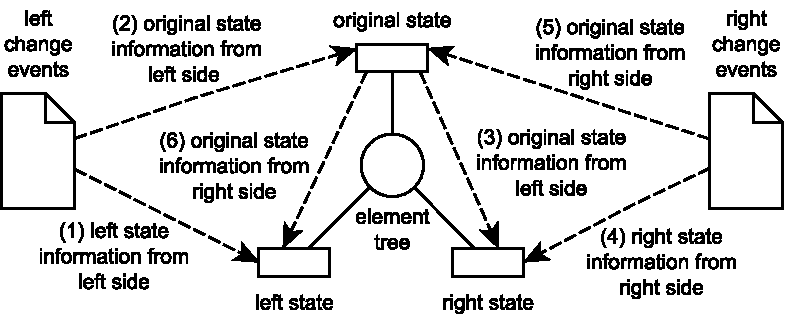
\includegraphics[width=\linewidth]{TreeConstruction}
    \caption{Steps in Element Tree construction.}
    \label{fig:tree_construction}
\end{figure}

\vspace{-20pt}
The construction of an element tree \textsf{elementTree} follows the steps Fig. \ref{fig:tree_construction}. First, the partial left state $S_{L}$ of a left model in the \textsf{elementTree} is constructed based on the information retrieved from the left change events (step 1). We denote this information as $I_{LL}$. We can also construct the partial state $S_{O}$ of the original version of the left model using the information related to the original state retrieved from the left change events $I_{OL}$ (step 2). Using the information $I_{OL}$, we can construct the partial state $S_{R}$ of the right model as a starting state before updating it during processing the right change events (step 3). Similarly, using the information from the right change events $I_{RR}$, we update the right state that has been initialised before using the information $I_{OL}$ (step 4). Thus,  $I_{OL} \cup I_{RR} \rightarrow S_{R}$. Also, information related to the partial state of the original model from the right change events is used to update the original state $I_{OR}$ (step 5). Thus, we have a more representative state of the original model using information from both sides, $I_{OL} \cup I_{OR} \rightarrow S_{O}$. The $I_{OR}$ is also used to update the left state to have a more representative partial state of the left model (step 6). Thus,  $I_{LL} \cup I_{OR} \rightarrow S_{L}$.   

\vspace{-10pt}
The \textsf{elementTree} construction conforms to the Alg. \ref{alg:element_tree}. Basically, it iterates through all a model's change events and uses the information contained in the change events to construct its partial state. The selection of side which side, left or right change events, that is executed first depends on the \textsf{Side} enumeration value -- \textsf{left} or \textsf{right} -- passed through the parameter \textsf{side} (the second input parameter). The algorithm also receives an input of the change events \textsf{events} that are to be iterated and the element tree \textsf{elementTree} that has been instantiated before, and then return the \textsf{elementTree} as output after updating it.

\IncMargin{1.5em}
\begin{algorithm}[H]
    \begin{footnotesize}
        \SetKwInOut{Input}{input}
        \SetKwInOut{Output}{output}
        \Input{a list of ChangeEvent $events$}
        \Input{an enumeration of Side $side$}
        \Input{an instance of ElementTree $elementTree$}
        \Output{an instance of ElementTree $elementTree$}
        \SetKwBlock{Beginn}{beginn}{ende}
        \Begin{
            \ForEach{$event$ in $events$}{
                $targetElement$ $\leftarrow$ getOrCreateNewTargetElement($event$, $elementTree$)\;
                $feature$ $\leftarrow$ getOrCreateNewFeature($event$, $targetElement$)\;
                $value$ $\leftarrow$ getValue($event$)\;
                $previousValue$ $\leftarrow$ getPreviousValue($event$)\;
                $position$ $\leftarrow$ getPosition($event$)\;
                $previousPosition$ $\leftarrow$ getPreviousPosition($event$)\;
                $featureEventList$ $\leftarrow$ getFeatureEventList($feature$, $side$)\;
                
                \BlankLine
                \tcp{put all values to their proper positions}
                updateTree($targetElement$, $feature$, $value$, $position$, $side$)\;
                $oldPosition$ $\leftarrow$ calculateOldPosition($featureEventList$, $previousPosition$, $side$)\;
                \If{\Not isCreated($value$, $side$) \And \Not isOldValueSet($feature$, $previousValue$, $previousPosition$, $side$)} {
                    setOldValue($feature$, $previousValue$, $oldPosition$, $side$)\;
                    $oppositeFeatureEventList$ $\leftarrow$ getOppositeFeatureEventList($feature$, $side$)\;
                    $oppositePosition$ $\leftarrow$ calculateOppositePosition($oppositeFeatureEventList$, $oldPosition$, $side$)\;
                    \If{\Not isDeleted($value$, $side$) \And \Not isOppositeSideValueSet($feature$, $value$, $oppositePosition$, $side$)} {
                        setOppositeSideValue($feature$, $value$, $oppositePosition$, $side$)\;
                    }
                }   
                
                addEventToFeatureEventList($event$, $featureEventList$)\;
                
            }
            \Return{$elementTree$}\;
        }
    \end{footnotesize}
    \caption{Algorithm to construct an element tree from events.}
    \label{alg:element_tree}
\end{algorithm}
\DecMargin{1.5em}

For each \textsf{event} in the \textsf{events}, we collect information needed to build up the \textsf{elementTree}  (lines 3-9), such as \textsf{targetElement}, \textsf{feature}, \textsf{value}, \textsf{previousValue}, \textsf{position}, and \textsf{previousPosition}. The \textsf{targetElement} is the element modified by a change event (e.g. \textsf{x} and \textsf{d} in List. \ref{lst:leftcbp}). This \textsf{targetElement} -- an instance of class Element in Fig. \ref{fig:approach_class_diagram} -- is retrieved from the \textsf{elementTree} if it already exists. Otherwise, a new one is created and added to the \textsf{elementTree} (line 3). In this step also we set the flags \textsf{*IsCreated} and \textsf{*IsDeleted} of the element in Fig. \ref{fig:approach_class_diagram}. For example, if the type of the event is \textsf{create} then \textsf{*IsCreated} is set to \textsf{true}. The \textsf{feature} -- an instance of class Feature in Fig. \ref{fig:approach_class_diagram} -- represents the target element's feature (e.g. \textsf{name} and \textsf{operations} in List. \ref{lst:leftcbp}) modified by a change event. It is  retrieved from the \textsf{targetElement}'s feature list, and a new one is created and added to the \textsf{targetElement}'s feature list if it has not existed yet (line 5). 

The \textsf{value} is the value assigned to the feature in a change event (line 5, Alg. \ref{alg:element_tree}). The \textsf{value} can be the type of \textsf{Element} (e.g. elements \textsf{b} and  \textsf{d}, lines 17-18, List. \ref{lst:leftcbp}) or primitive (e.g. the String ``MathLib'' at line 14 in the List. \ref{lst:leftcbp}). The \textsf{previousValue} is similar to the \textsf{value} except that it represents the previous value of the modified feature (line 6, Alg. \ref{alg:element_tree}). The \textsf{previousValue} is not defined if there is no previous value has been assigned. If the type of \textsf{value} and \textsf{previousValue} is \textsf{Element}, the elements that they represent are retrieved from the \textsf{elementTree} otherwise new instances are created if they are contained yet in the \textsf{elementTree}. Not every change event has \textsf{value}, particularly event with type \textsf{add} or \textsf{delete} as it only modifies a target element not the element's feature.

The \textsf{position} is the position assigned by a change event to a value in a feature, while \textsf{previousPosition} is the previous position of the value (lines 7-8, Alg. \ref{alg:element_tree}). In one change event, we can get both \textsf{position} and \textsf{previousPosition} or only one of them depends on the type of the change event. For example, we can only obtain that the \textsf{position} of \textsf{d} is 1 (line 17 in in the List. \ref{lst:leftcbp}) as the change event type is \textsf{add}. In \textsf{remove} change event, we can only get the \textsf{previousPosition} of \textsf{b}, that is 2 (line 17 in in the List. \ref{lst:leftcbp}), as the element does not exist anymore in the left model. We can obtain both of them only in a \textsf{move} change event as an element is moved from a previous position to a new one (line 14 in in the List. \ref{lst:rightcbp}). For a single-valued feature, the \textsf{position} and \textsf{previousPosition} are always 0 as the feature can only contain a value. 

At line 9, we retrieve the \textsf{featureEventList} from the \textsf{feature} to be added later with the current \textsf{event} (line 19). The \textsf{featureEventList} is a list -- a history -- of change events that have been processed that are specific to the \textsf{feature} on the selected \textsf{side}. Using the obtained \textsf{targetElement}, \textsf{feature}, \textsf{value}, and \textsf{position}, the process then updates the state of the \textsf{elementTree} on the selected \textsf{side} (line 10). After that, it calculates back the original position of a value using the \textsf{featureEventList} and \textsf{previousPosition} (line 11). If the value at \textsf{oldPosition} in the \textsf{feature} has not been set, then the algorithm sets the \textsf{feature} with the \textsf{previousValue} at the \textsf{oldPosition} in the partial state of the original model (lines 12-13). At lines 14-18, the algorithm also does the same thing to the opposite side -- if the current \textsf{side} is \textsf{left} then it is \textsf{right}.  

To better understand how the algorithm works, we explain its execution using both change events in the Listings \ref{lst:leftcbp} and \ref{lst:rightcbp}. We start from the left change events. 

\vspace{-10pt}
\subsubsection{Left Side.}\label{sec:left_side} In List. \ref{lst:leftcbp}, the first event is a \textsf{session} event (line 13). \textsf{Session} event indicates that its following events -- until the next session event or end of file -- are one batch of changes when they were persisted into a change-based persistence file. This event is not significant for model comparison; thus it is skipped. 

\begin{wrapfigure}[37]{r}{0.5\textwidth}
    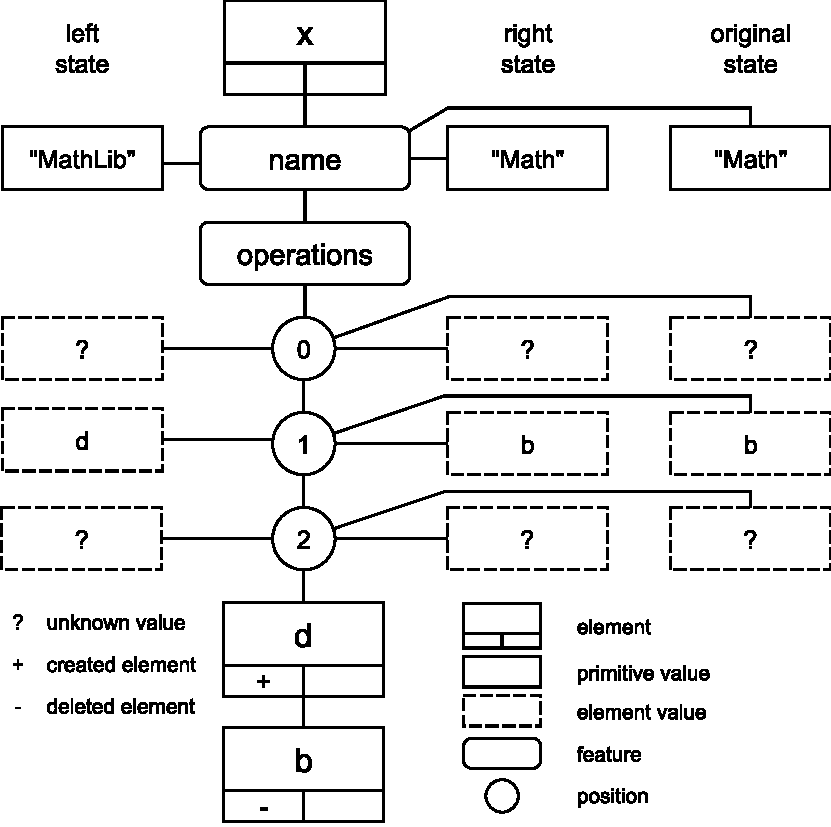
\includegraphics[width=\linewidth]{LeftElementTreeDiagram}
    \caption{The \textsf{elementTree} after processing all left change events.}
    \label{fig:left_element_tree_diagram}
    \vspace{1em}
    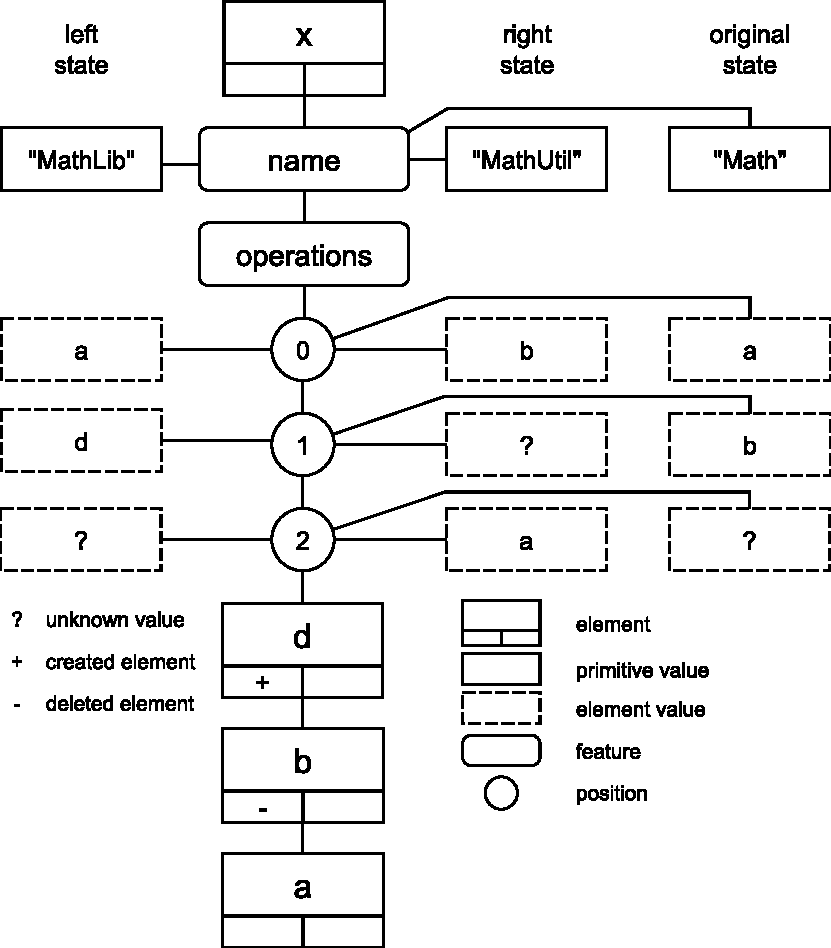
\includegraphics[width=\linewidth]{RightElementTreeDiagram}
    \caption{The \textsf{elementTree} after processing all left and right change events.}
    \label{fig:right_element_tree_diagram}
\end{wrapfigure}

In the next event [\texttt{\small \textbf{set} x.name \textbf{from} "Math" \textbf{to} "MathLib"}] at line 14, we can identify that there is an element with id \textsf{x} that has been existed from the original model. It has a feature \textsf{name} with a value ``Math'' in the original model and has been changed to ``MathLib'' in the left model. Since the element \textsf{x} has not existed in the \textsf{elementThree}, we create its instance of \textsf{Element} and also its feature \textsf{name}. We set the value of the feature \textsf{name} to ``MathLib'' and also set it to ``Math'' in the partial state of the original model -- it has not been set before. As this feature on the right side also has not been set, we set it to ``Math'' as well. Once a feature in the original state has been set, it cannot be overridden -- using the flag \textsf{isOldSet} in class \textsf{Feature} in Fig. \ref{fig:approach_class_diagram}. 

In the event [\texttt{\small \textbf{create} d \textbf{type} Operation}] at line 15, we can identify that there an element with id \textsf{d} has been created. We also update the \textsf{elementTree} to include this element and set the element's flag \textsf{leftIsCreated} to \textsf{true}. In the event [\texttt{\small \textbf{set} d.name \textbf{to} "sqrt"}] at line 16, we can identify that element \textsf{d}'s feature \textsf{name} has been set to ``sqrt''. Thus, we update the \textsf{d}'s feature \textsf{name} in the \textsf{elementTree}. From the event [\texttt{\small \textbf{add} d \textbf{to} x.operations \textbf{at} 1}] at line 17, we can deduce that element \textsf{d} is added to position 1 in the element \textsf{x}'s feature \textsf{operations}. Thus, we assign \textsf{d} to element \textsf{x}'s feature \textsf{operations} at position 1 in the \textsf{elementTree}. As \textsf{d} is a new element that only exists in the left model, we do not update changes of this element to the original and right models. 

From the event [\texttt{\small \textbf{remove} b \textbf{in} x.operations \textbf{at} 2}] at line 18, we can identify that there is element \textsf{b} in the original model, but it is deleted in the left model. The position of element \textsf{b} in the original model is calculated by comparing its previous position to the previous change events that have been applied to its feature and increase or decrease it depending on the conditions with the previous change events (the previous change events are obtained from $changeEventList$ in Alg. \ref{alg:element_tree}). Since the previous event is adding element \textsf{d} to position 1 and the position of \textsf{b} is at 2 at the time it is removed, we can deduce that before element \textsf{d} is added, the position of element \textsf{b} is at 1 and shifted to 2 because of the addition of element \textsf{d}.  Therefore, we can conclude that the original position of element \textsf{b} is at 1. Thus, we update the original state of the \textsf{elementTree} by adding element \textsf{b} into the element \textsf{x}'s feature \textsf{operations} at position 1.  



We perform the same procedure to also add element \textsf{b} to the right state of the \textsf{elementTree}. However, since there is no change event has been applied to right side of element \textsf{x}'s feature \textsf{operations}, the calculation of element \textsf{b}'s position should return the same value as in the original state (line 15, Alg. \ref{alg:element_tree}), and thus element \textsf{b} has the same position as in the original state. It is important to notice, in this step, the flag \textsf{isRightSet} (class \textsf{Feature}, Fig. \ref{fig:approach_class_diagram}) is not set to \textsf{true} since we want the value can be overridden during processing the right change events. The last event [\texttt{\small \textbf{delete} b}], removes the element \textsf{b} from the left model. Hence, we set the flag \textsf{isLeftDeleted} of element \textsf{a} to \textsf{true}.

Fig. \ref{fig:left_element_tree_diagram} illustrates the state of the \textsf{elementTree} after all left change events have been processed. As can be seen, the \textsf{elementThree} exhibits the partial states of the original, left, and right models at once. 

\vspace{-10pt}
\subsubsection{Right Side.}\label{sec:right_side}  Similar to the left side, the List. \ref{lst:rightcbp} also starts with a \textsf{session} event (line 13) indicating a new batch of change events. From the event [\texttt{\small \textbf{move} a \textbf{in} x.operations \textbf{from} 0 \textbf{to} 2}] at line 14, we can infer that in the right model there is an element with id \textsf{a} positioned at 2 in the element \textsf{x}'s feature \textsf{operations}. Thus, an instance of class \textsf{Element} of this element \textsf{a} is added to the \textsf{elementTree} and positioned at index 2 of the element \textsf{x}'s feature \textsf{operations}. Since the event is a \textsf{move} type and the new position is larger than its previous position, it means elements that are between its previous and new positions are shifted one place down. As element \textsf{b} has already existed in the same feature (the element was added during the process of the left change events) and its position is between element \textsf{a}'s movement, the position of element \textsf{b} is shifted down from 1 to 0. 

Also since the event's type is \textsf{move} and its previous position is 0 and it is the first event that changes the position of element \textsf{a}, these conditions imply that element \textsf{a} in original model is positioned at 0 in the element \textsf{x}'s feature \textsf{operations}. Therefore, we add the element \textsf{a} to  the element \textsf{x}'s feature \textsf{operations} in the original state of the \textsf{elementTree}. Since the position 0 in the element \textsf{x}'s feature \textsf{operations} has not been set, we also add element \textsf{a} to that position in the right state of the \textsf{elementTree}. From the last event [\texttt{\small \textbf{set} a.name \textbf{from} "Math" \textbf{to} "MathUtil"}] at line 15, we can infer that in the right model the value of element \textsf{a}'s feature \textsf{name} is ``MathUtil'' in the right model. Hence, we set the feature \textsf{name} to ``MathUtil'' in the right state. We do apply this operation to the original and left states as they have been set before.  

Fig. \ref{fig:right_element_tree_diagram} exhibits the state of the \textsf{elementTree} after both side change events have been processed. Using this data structure, we can determine the difference between the left and right models without having to visit and compare all elements and features of both models, which we discuss in the next section.

\subsection{Diff Computation}
\label{sec:diff_computation}

\IncMargin{1.5em}
\begin{algorithm}[H]
    \begin{footnotesize}
        \SetKwInOut{Input}{input}
        \SetKwInOut{Output}{output}
        \Input{an instance of ElementTree $elementTree$}
        \Begin{
            $diffList$ $\leftarrow$  DiffList()\;
            \ForEach{$element$ \In $elementTree$}{
                \ForEach{$feature$ \In getFeatures($element$)}{
                    \ForEach{$position$ \In getPositions($feature$)}{
                        $leftValue$ $\leftarrow$ getLeftValue($feature$, $position$)\;
                        $rightValue$ $\leftarrow$ getRightValue($feature$, $position$)\;
                        \BlankLine
                        \tcp{rules starts from here}
                        $diffs$ $\leftarrow$ identifyDiffUsingRules($element$, $feature$, $leftValue$, $rightValue$, $position$)\;
                        addToDiffList($diffs$,$diffList$)\;
                    }
                }
            }
            \Return{$diffList$}\;
        }
    \end{footnotesize}
    \caption{Algorithm to determine differences.}
    \label{alg:diff_calculation}
\end{algorithm}
\DecMargin{1.5em}

After the \textsf{elementTree} has been constructed, we iterate through elements and features of the \textsf{elementTree} and use the flags, containers, containing features, and positions on both sides of each element and value to identify differences between both left and right models. Basically, we follow the steps in Alg. \ref{alg:diff_calculation}. The algorithm works by visiting each element and every position of each its features (lines 3-5). At every position, it retrieves the \textsf{leftValue} and \textsf{rightValue} (lines 5-7).  Both together with the \textsf{element}, \textsf{feature}, and \textsf{position} are passed to a function \textsf{identifyDiffUsingRules} (line 8). The function identify differences by using a set of pre-defined rules which determines differences \textsf{diffs} based on the conditions of the flags of \textsf{element}, attributes of \textsf{feature}, both \textsf{*Values}, and \textsf{position}. The obtained \textsf{diffs} are then added to the overall list of differences \textsf{diffList} which returned as an output (line 8-9, 13). 

Since we use a great number of rules in our implementation, we only discuss rules that we use to identify differences in the running example, as presented in Table \ref{table:diff_rules}. It is important to remember that we use the left model as a reference which means the differences are presented as changes that transform the right model to become equal to the left model. For example, if the type of difference is \textsf{ADD}, it means that a value exists in the left model but does not exist in the right model. During the iteration of the \textsf{elementTree} in Fig. \ref{fig:right_element_tree_diagram}, when the iteration is at feature \textsf{name}, as the type of this feature is a single-valued attribute, to make the left value of this feature equals to the right value is by overriding the value ``MathUtil'' with ``MathLib''. Thus, the type of this difference is \textsf{CHANGE} (fourth column, Table \ref{table:diff_rules}).

When the iteration is at position 0 in the element \textsf{x}'s feature \textsf{operations}, we have two values: the \textsf{leftValue} is element \textsf{a}, and the \textsf{rightValue} is element \textsf{b}. For element \textsf{a}, as it exists on both sides -- all flags \textsf{*Created} and \textsf{*Deleted} are false, we process this element later at its largest position (element \textsf{a}'s \textsf{leftPositon} < \textsf{rightPositon}). For element \textsf{b}, since it has been deleted from the left state (flag \textsf{isLeftDeleted} = true) and still exists in the right state (flag \textsf{isRightDeleted} = false) then to make element \textsf{b} does not exist in the right state is by deleting it. Thus, the type of this difference is \textsf{DELETE} (first column, Table \ref{alg:diff_rules}).

\IncMargin{1.5em}
\begin{algorithm}[H]
    \begin{footnotesize}
        \SetKwInOut{Input}{input}
        \SetKwInOut{Output}{output}
        \Input{an Element $element$, a Feature $feature$, a variable $leftValue$, a variable $rightValue$, an Integer $position$}
        \Output{a List of Diff $position$}
        $diffs$ $\leftarrow$ createDiffList()\;
        \tcp{...}
        \tcp{rightValue}
        \tcp{Rule 1: one of rules to determine deletion of an element}
        \If{getType($feature$) \Is Containment \And leftIsCreated($rightValue$)\Is false \And leftIsDeleted($rightValue$) \Is true \And rightIsCreated($rightValue$) \Is false \And rightIsDeleted($rightValue$) \Is false}{
             createNewDiff(getLeftContainer($rightValue$), getRightContainer($rightValue$), getLeftFeature($rightValue$), getRightFeature($rightValue$), getLeftPosition($rightValue$), getRightPosition(), rightValue, null, DifferenceType.DELETE)\;
            addDiffToDiffList($diff$, $diffs$)\;
       }
        \tcp{leftValue}
        \tcp{Rule 2: one of rules to determine addition of an element}
        \If{getType($feature$) \Is Containment \And leftIsCreated($leftValue$)\Is true\And leftIsDeleted($leftValue$) \Is false \And rightIsCreated($leftValue$) \Is false \And rightIsDeleted($leftValue$) \Is false}{
            $diff$ $\leftarrow$ createNewDiff(getLeftContainer($leftValue$), getRightContainer($leftValue$), getLeftFeature($leftValue$), getRightFeature($leftValue$), getLeftPosition($leftValue$), getRightPosition($leftValue$), null, rightValue, DifferenceType.ADD)\;
            addDiffToDiffList($diff$, $diffs$)\;
        }
        \tcp{Rule 3: one of rules to determine movement of an element}
        \If{getType($feature$) \Is Containment \And leftIsCreated($leftValue$)\Is false \And leftIsDeleted($leftValue$) \Is false \And rightIsCreated($leftValue$) \Is false \And rightIsDeleted($leftValue$) \Is false \And (getLeftContainer($leftValue$) <> getRightContainer($leftValue$) \Or getLeftFeature($leftValue$) <> getRightFeature($leftValue$) \Or getLeftPosition($leftValue$) <> getRightPosition($leftValue$)}{
            $diff$ $\leftarrow$ createNewDiff(getLeftContainer($leftValue$), getRightContainer($leftValue$), getLeftFeature($leftValue$), getRightFeature($leftValue$), getLeftPosition($leftValue$), getRightPosition($leftValue$), leftValue, leftValue, DifferenceType.MOVE)\;
            addDiffToDiffList($diff$, $diffs$)\;
        }
        \tcp{Rule 4: a rule to determine a change of a single-valued attribute}
        \If{getType($feature$) \Is Attribute \And isSingleValued($feature$) \And leftValue <> rightValue}{
            $diff$ $\leftarrow$ createNewDiff($element$, $element$, $feature$, $feature$, $position$, $position$, $leftValue$, $rightValue$, DifferenceType.CHANGE)\;
            addDiffToDiffList($diff$, $diffs$)\;
        } 
        \tcp{...}
        \Return{$diffList$}
    \end{footnotesize}
    \caption{Some rules to determine differences.}
    \label{alg:diff_rules}
\end{algorithm}
\DecMargin{1.5em}



We can get only one value when the iteration is at position 1 in the element \textsf{x}'s feature \textsf{operations}; the \textsf{leftValue} is element \textsf{b}, but the \textsf{rightValue} is unidentified. Thus we only process the \textsf{leftValue}. Element \textsf{d} is created only in the right state. Thus, to make element \textsf{d} also exists in right state is by adding it into element \textsf{x}'s feature \textsf{operations} at position 1. Therefore, the type of this difference is \textsf{ADD} (second column, Table \ref{table:diff_rules}). 

At position 2, we only have one value; the \textsf{leftValue} is unidentified, and the \textsf{rightValue} is element \textsf{a}. Since element \textsf{a} has different positions in both states, at 0 in the left state and 2 in the right state. We can conclude that in order to make the position of element \textsf{a} in right state equals its position in the left state, element \textsf{a} should be moved from position 2 to 0. Thus, the type of this difference is \textsf{MOVE} (third column, Table \ref{table:diff_rules}).

We formulate the identified differences as $dc_{n}$ = [$LeftContainer_n$, $RightContainer_n$, $LeftFeature_n$, $RightFeature_n$, $LeftPosition_n$, $RightPosition_n$, $LeftValue_n$, $RightValue_n$, $Kind_n$] to its state-based counterpart in the end part of Section \ref{sec:model_comparison}. Thus, $dc_{1}$ =  [\textsf{x}, \textsf{x}, \textsf{name}, \textsf{name}, 0, 0, ``MathLib'', ``Mathutil'', \textsf{CHANGE}], $dc_{2}$ = [\textsf{x}, \textsf{x}, \textsf{operations}, \textsf{operations}, ?, 0, ?, \textsf{b}, \textsf{DELETE}], $dc_{3}$ = [\textsf{x}, \textsf{x}, \textsf{operations}, \textsf{operations}, 1, ?, \textsf{d}, ?, \textsf{ADD}], and $dc_{c4}$ = [\textsf{x}, \textsf{x}, \textsf{operations}, \textsf{operations}, 0, 2, \textsf{a}, \textsf{a}, \textsf{MOVE}]. As can be noticed, this change-based approach might produce differences that are different from differences that the state-based approach produces which can be seen between  $ds_{4}$ and $dc_{4}$ ($ds_{4}$ $\neq$ $dc_{4}$). In the state-based approach, the difference is the element \textsf{c} is in different positions while in the change-based approach this difference is attributed to element \textsf{a}. However, for both approaches, if we resolve their differences to make the right model equals to the left model -- executing all-left-to-right merging, the right model becomes equal to the left model. In this way, we can check the correctness of the identified differences produced by the change-based approach.

\section{Evaluation Method}
\label{sec:evaluation}

In order to evaluate the performance of the change-based approach in comparing models, we have evaluated it against the traditional state-based approach as the benchmark. We choose EMF Compare \cite{emfcompare2018developer,eclipse2017compare} as the tool to perform the state-based comparison since it is a common tool to compare EMF-based models. Since we could not find any existing large models persisted in change-based format to be used as the dataset for our experiments, we reverse-engineered a large model -- it confirms the Java metamodel \cite{eclipse2018modiscojava} -- from the Epsilon project \cite{eclipse2018epsilongit,eclipse2017epsilon}. The model consists of more than 1.6 million elements with a size of 224 MBs persisted in XMI format. 

We cloned the original model to produce two new -- left and right -- models and perform random changes -- random operations (e.g. add, remove, move, set) with random elements, features, positions, and values -- to both models to create differences between them. Since we wanted the change of total elements did not affect our measurement, the probabilities of executing \textit{add} and \textit{remove} operations were made equal. Thus, the total number of elements can be kept constant, and the modification can still include both operations. We made 1.1 million changes to each model which generated more than 1.1 million events (one operation can generate more than one event, e.g. a \textit{move} between features generates \textit{remove} and \textit{add} events). Events generated by the changes were persisted in change-based format (to be used later in change-based model comparison). After every 50 thousand changes, we also persisted the last state of the models in state-based format (to be used later in state-based model comparison) and then performed the change-based and state-based model comparison and measured their comparison time and memory footprint, thus produced 22 records of measurement. 

Since the change-based and state-based approaches can produce different differences, in order to evaluate the correctness of the change-based approach, we reconciled all the differences by performing all-left-to-right merging -- making the right model identical to the left model -- based on the identified differences. If the all-left-to-right merging of change-based approach produces a model that is identical to the model produced by the all-left-to-right merging of the state-based approach then it can be said that differences identified by the change-based approach are correct. We performed this correctness checking at every time the measurement mentioned above was executed.

\section{Result and Discussion}
\label{sec:discussion}

Fig. \ref{fig:modification_model_size} depicts the modification course stated in Section \ref{sec:evaluation}. The increase of events correlates positively to the number of affected elements and differences. As the number of events inclines, the probability of changes that modify already-affected elements or features also gets higher. Thus, some changes might not contribute to the addition of new affected elements or differences -- more changes are required to add or create new elements or differences. In consequence, both grow in a logarithmic manner as can be seen in Fig. \ref{fig:modification_course}. As designed in Section \ref{sec:evaluation}, the number of total elements of both models is almost constant. The total of elements of both models does change but in the order of hundreds (in contrast, both models have more than 3.2 million in total). Fig. \ref{fig:model_size} depicts the zoom-in view of the total elements in Fig. \ref{fig:modification_course}.

\begin{figure}[ht]
    \centering
    \begin{subfigure}[t]{0.495\linewidth}
        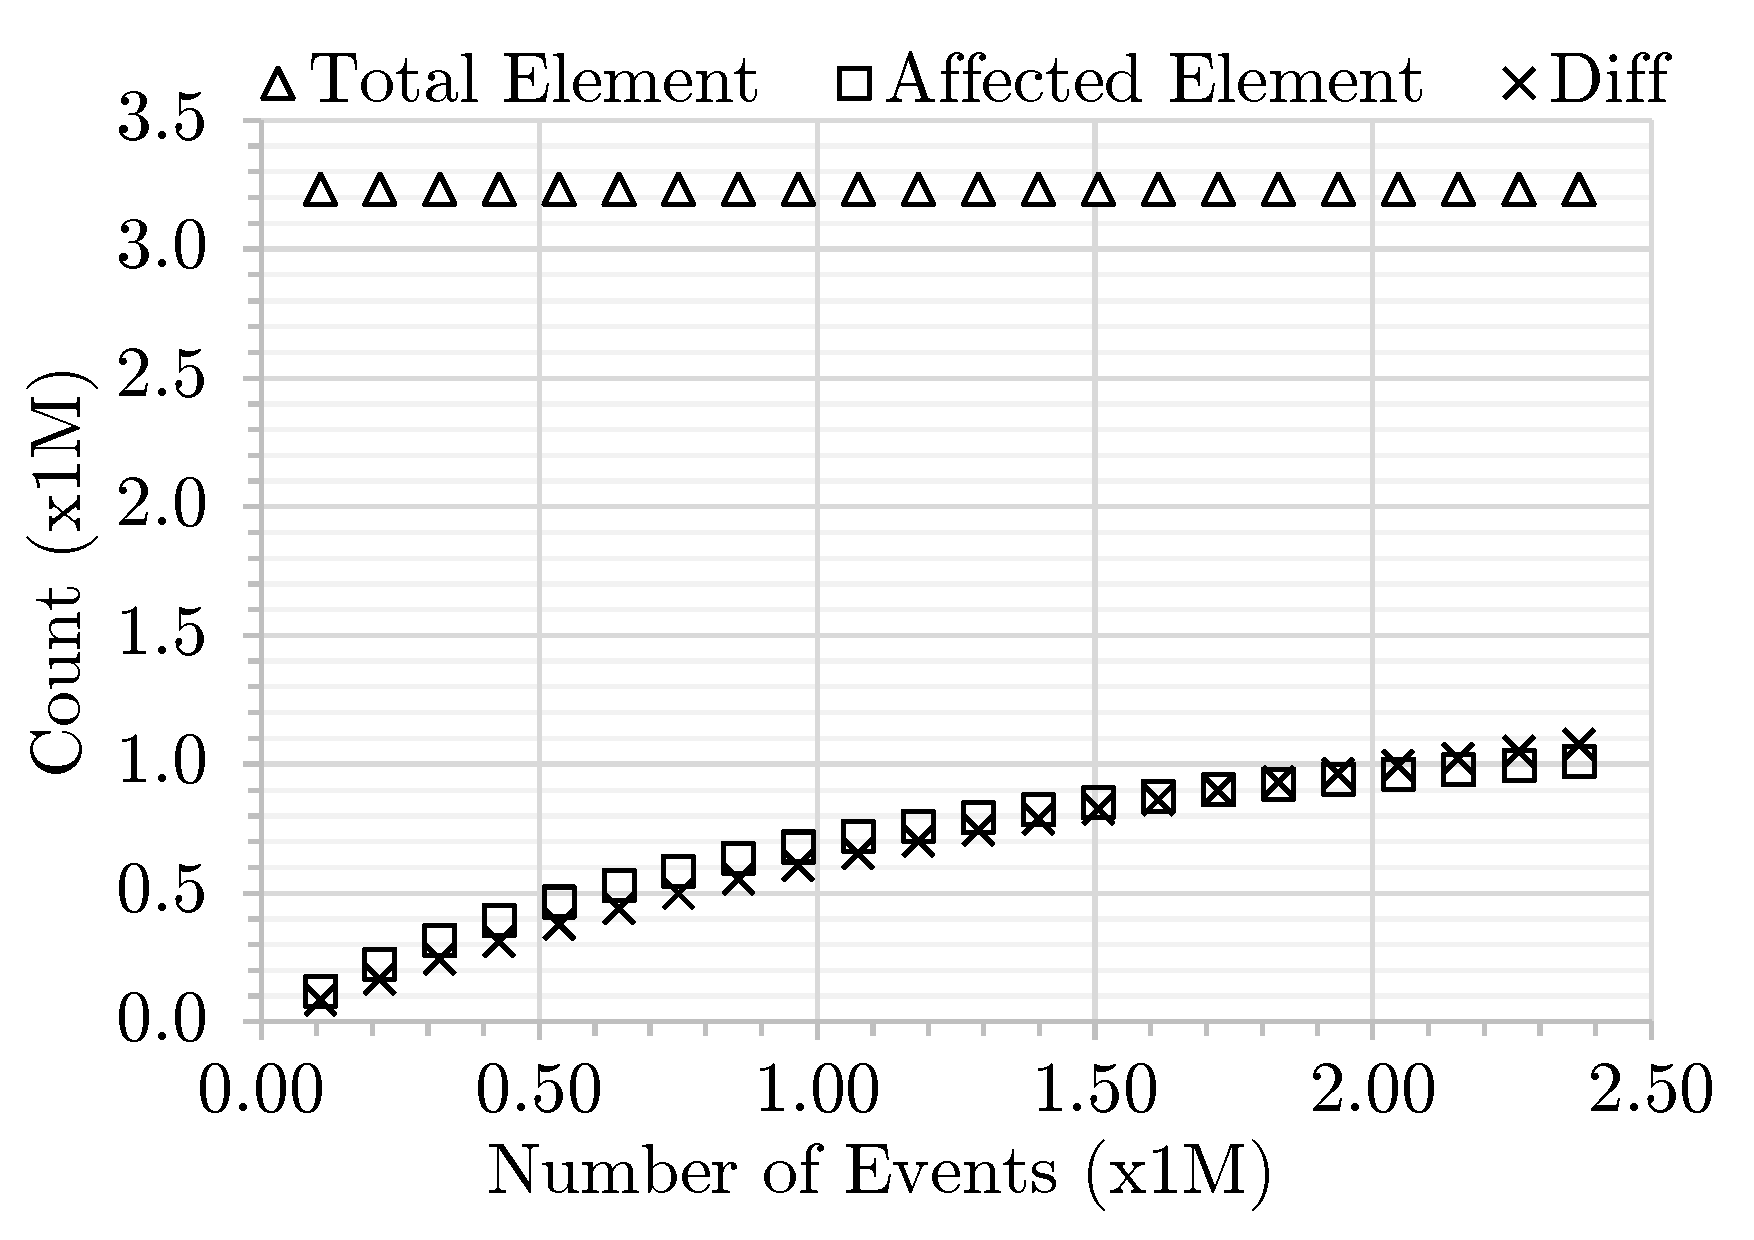
\includegraphics[width=\linewidth]{ModificationCourse}
        \caption{total elements, affected elements, and diffs}
        \label{fig:modification_course}
    \end{subfigure}
    \hfill
    \begin{subfigure}[t]{0.495\linewidth}
        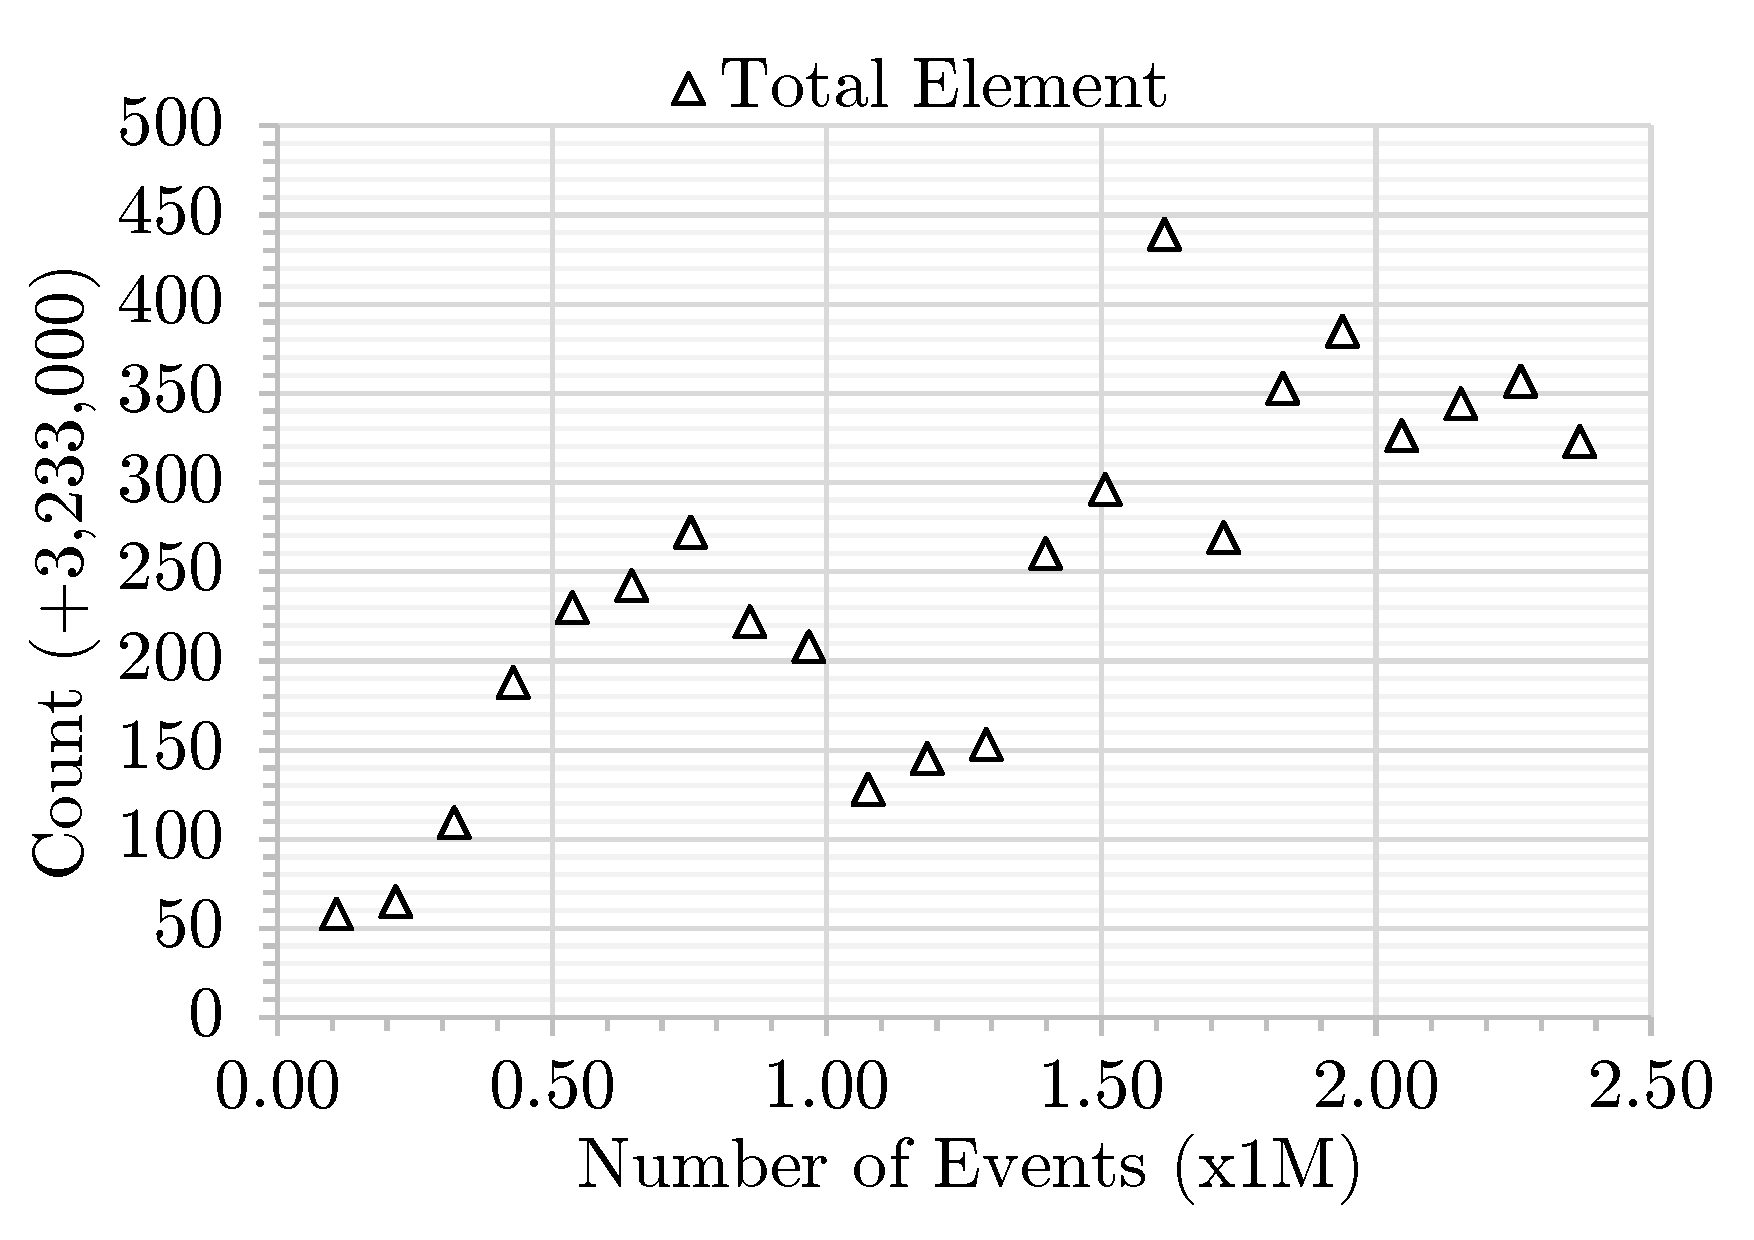
\includegraphics[width=\linewidth]{ModelSize}
        \caption{zoom-in view of total elements in Fig. \ref{fig:modification_course}}
        \label{fig:model_size}
    \end{subfigure}
    \caption{Changes on models along the artificial modification.}
    \label{fig:modification_model_size}
\end{figure}

\begin{figure}[ht]
    \centering
    \begin{subfigure}[t]{0.495\linewidth}
        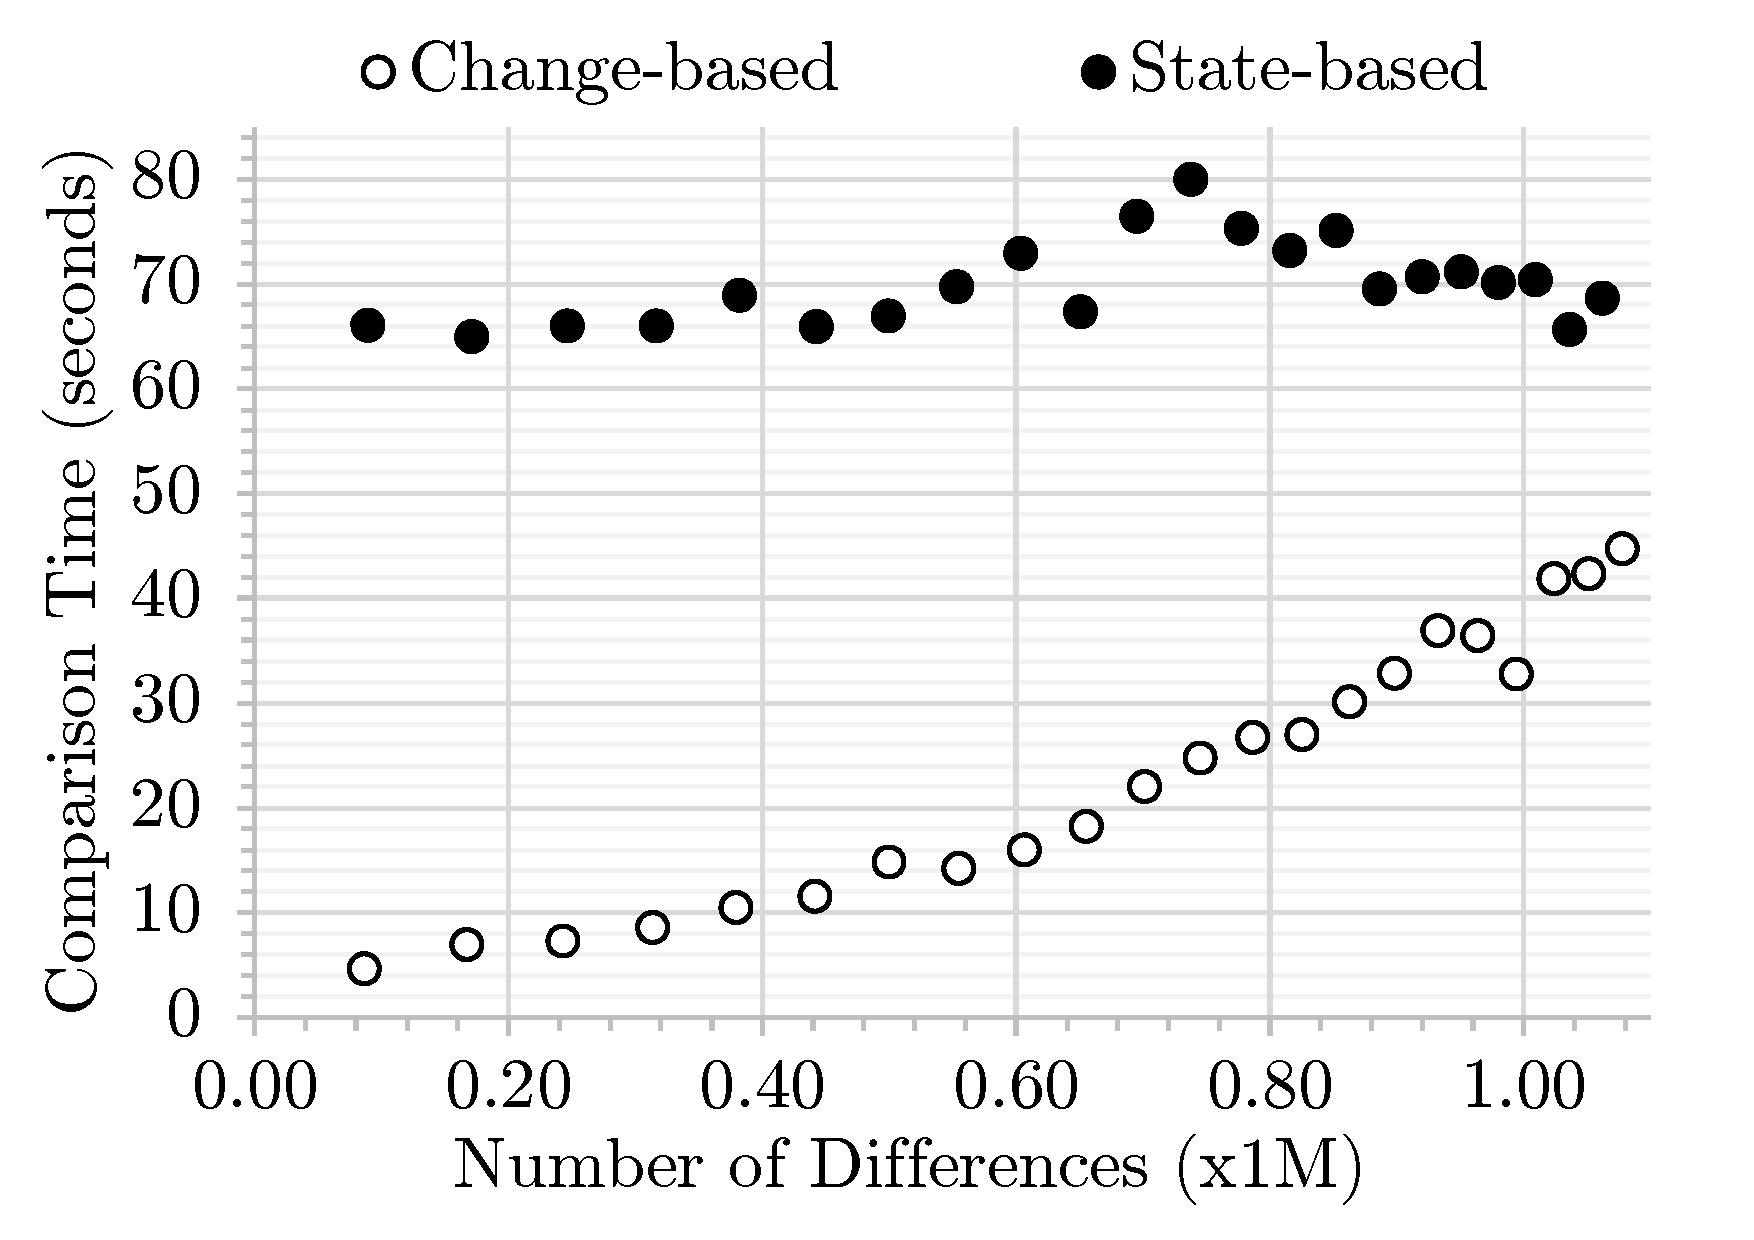
\includegraphics[width=\linewidth]{Time-Diffs}
        \caption{execution time}
        \label{fig:time_diffs}
    \end{subfigure}
    \hfill
    \begin{subfigure}[t]{0.495\linewidth}
        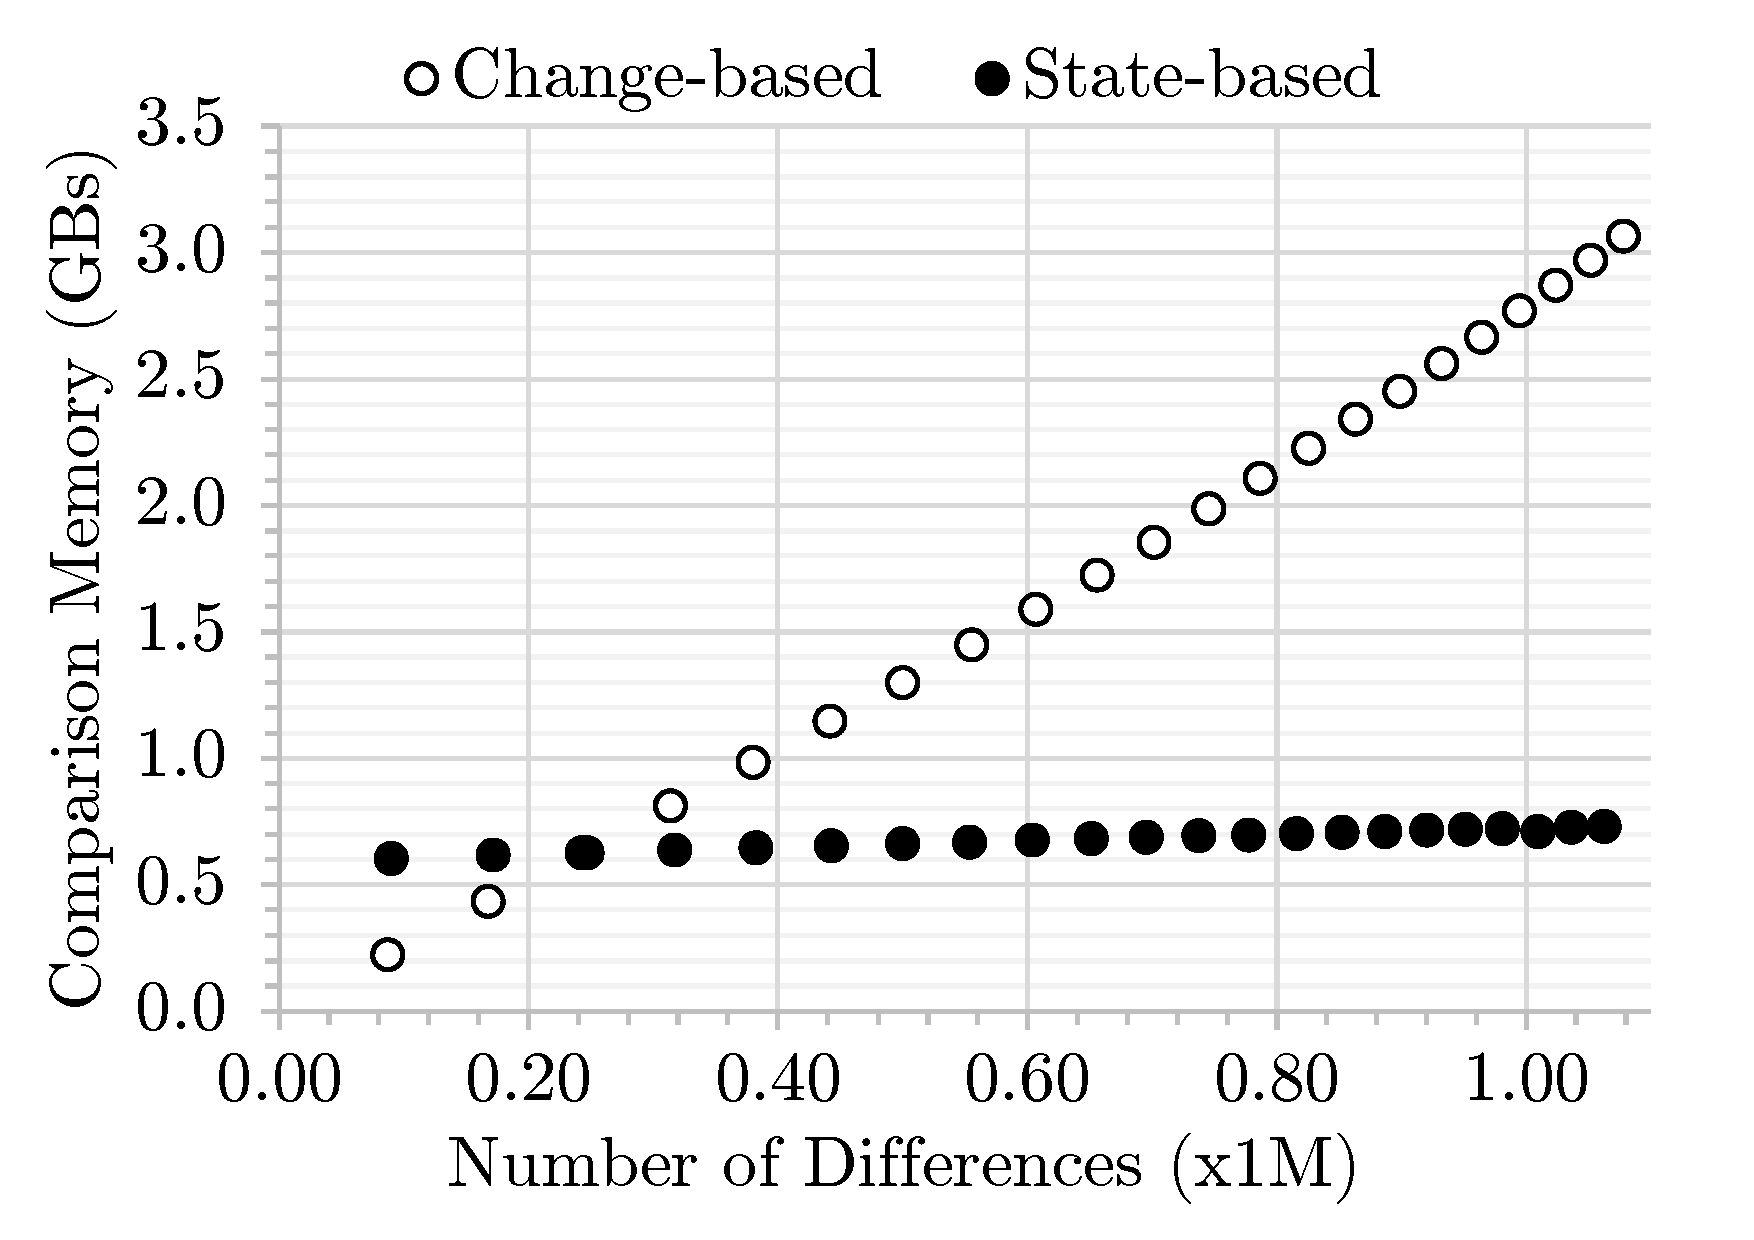
\includegraphics[width=\linewidth]{Memory-Diffs}
        \caption{memory footprint}
        \label{fig:memory_diffs}
    \end{subfigure}
    \caption{Change-based vs. state-based model comparison as differences increase.}
    \label{fig:change_vs_state}
\end{figure}

Figures \ref{fig:time_diffs} and \ref{fig:memory_diffs} show the execution time and memory footprint of the change-based and state-based comparison to contrast their performance. We can notice that the change-based comparison outperforms the state-based comparison regarding of execution time. The change-based approach only requires 5 seconds compared to the state-based approach that takes 66 seconds to identify around 90,000 differences (see the first circles). However, as the number of differences grows -- which also indicates increase on events, a growing number of events also have to loaded also into memory for the construction of the element three thus slows down the comparison. Fig. \ref{fig:time_changediff_detail} breaks down the comparison time in detail. It exhibits that the event loading time is the dominant contributor to the slowdown compared to the element tree's construction time and diffing time -- the diffing time is the weakest contributor. 

\begin{figure}[ht]
    \centering
    \begin{subfigure}[t]{0.495\linewidth}
        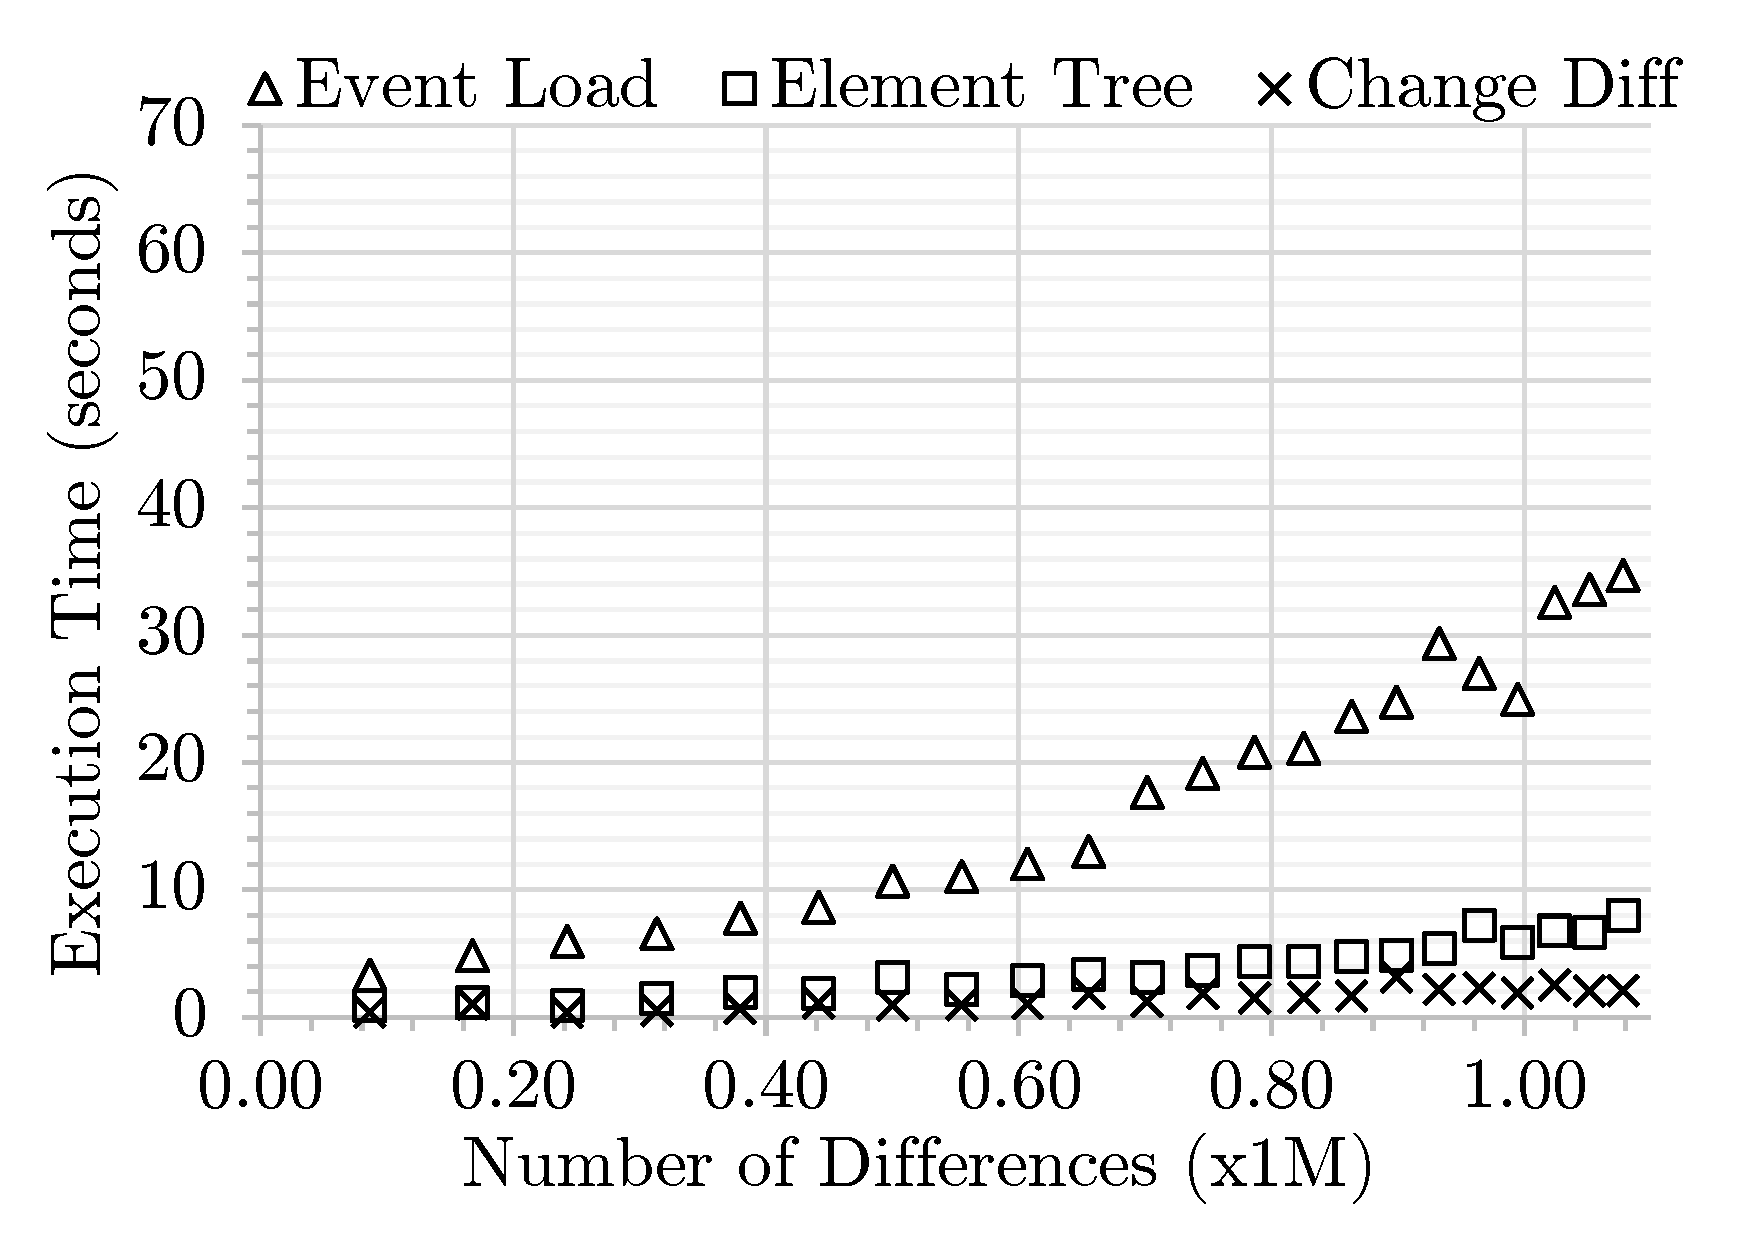
\includegraphics[width=\linewidth]{Time-ChangeDiff-Detail}
        \caption{change-based execution time}
        \label{fig:time_changediff_detail}
    \end{subfigure}
    \hfill
    \begin{subfigure}[t]{0.495\linewidth}
        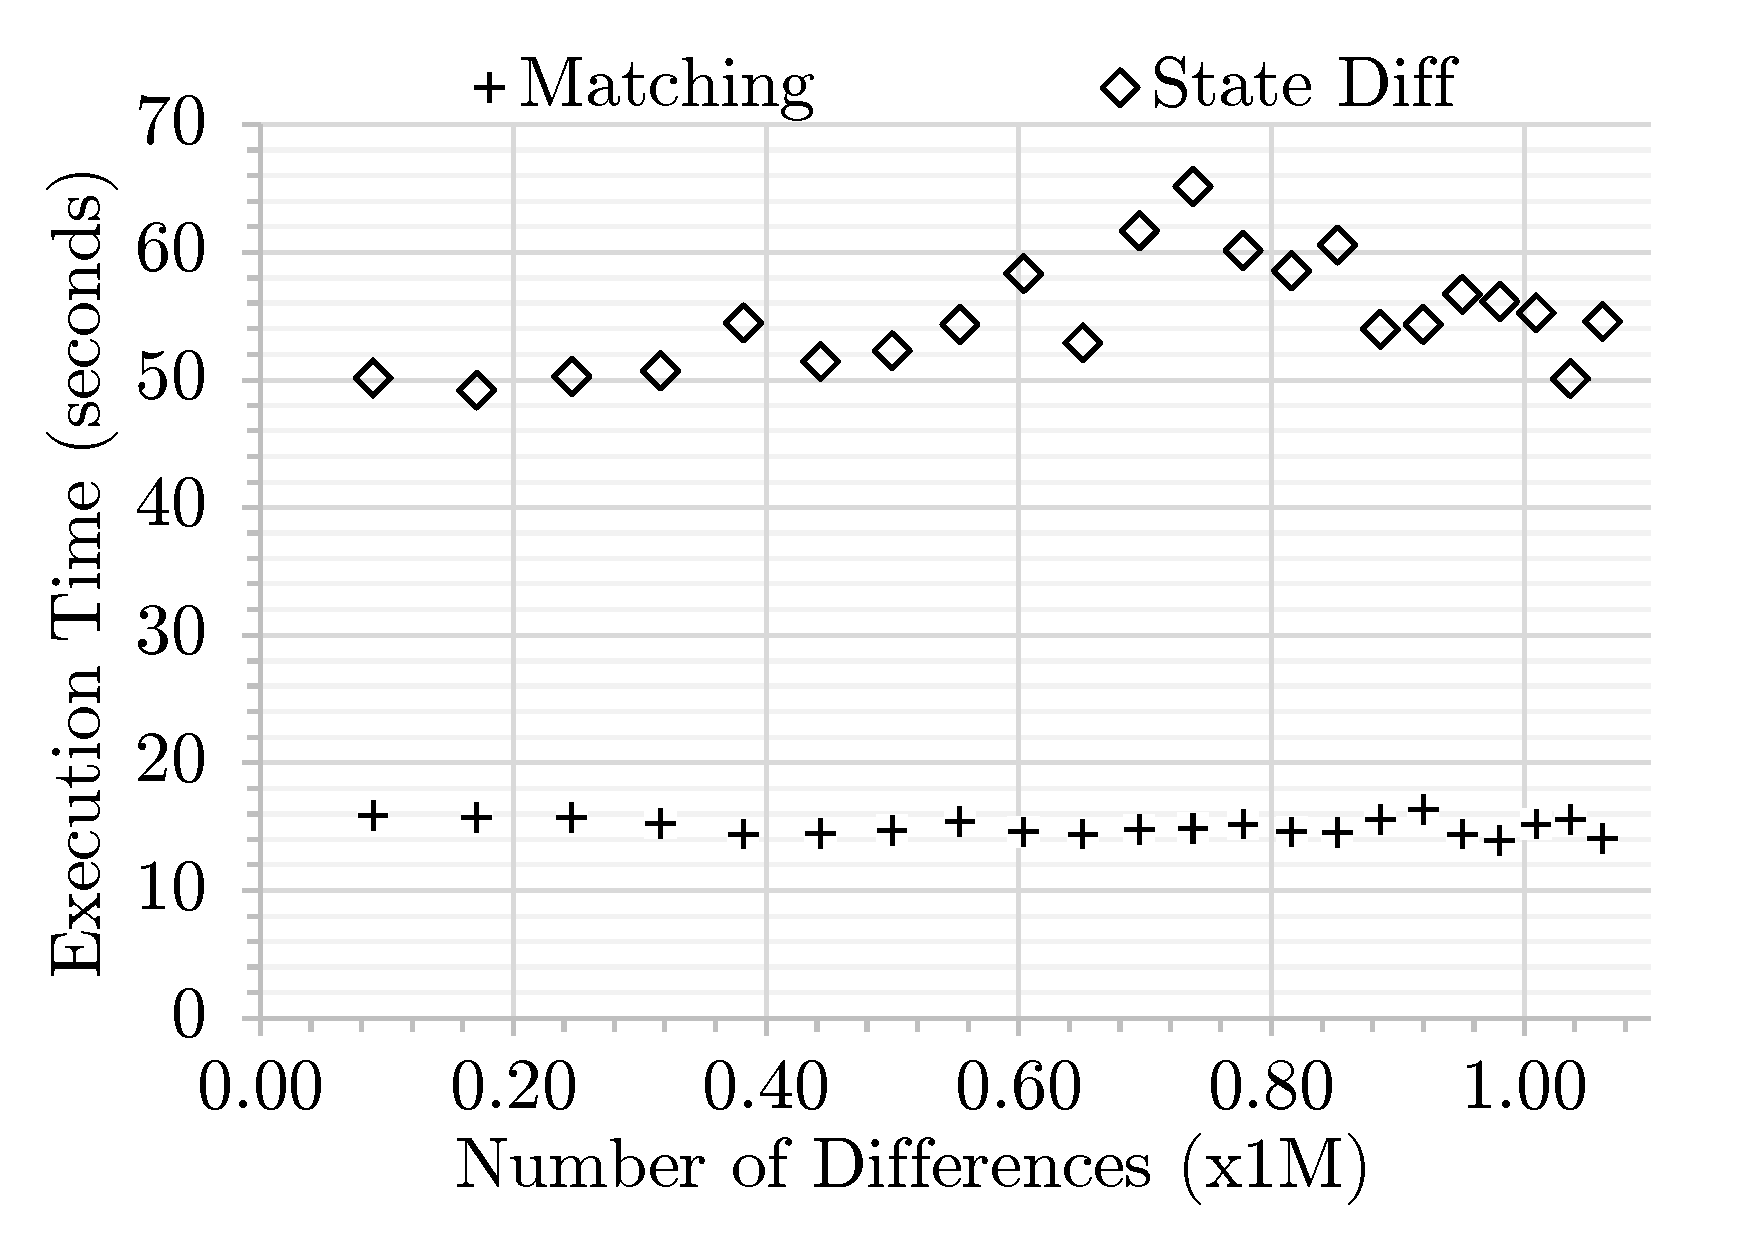
\includegraphics[width=\linewidth]{Time-StateDiff-Detail}
        \caption{state-based execution time}
        \label{fig:time_statediff_detail}
    \end{subfigure}
    \begin{subfigure}[t]{0.495\linewidth}
        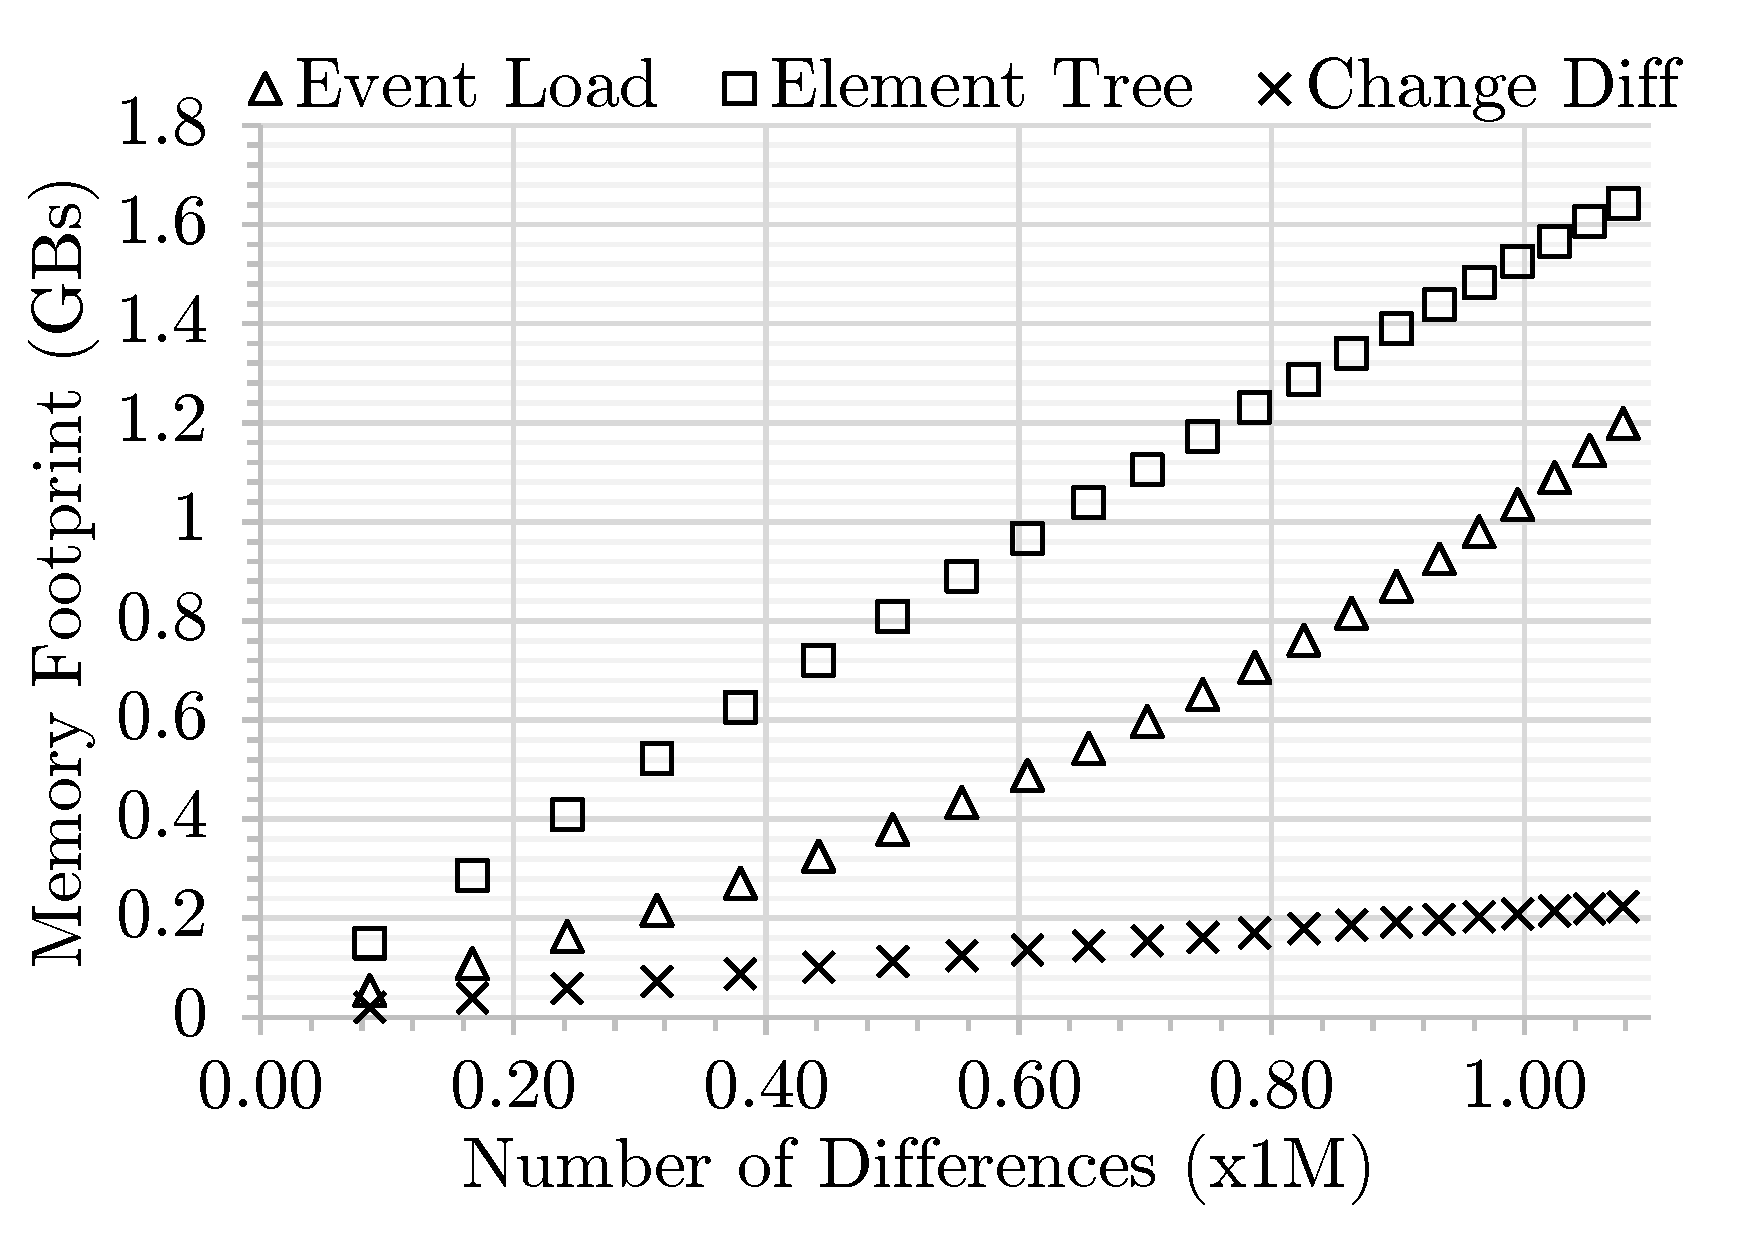
\includegraphics[width=\linewidth]{Memory-ChangeDiff-Detail}
        \caption{change-based memory footprint}
        \label{fig:memory_changediff_detail}
    \end{subfigure}
    \hfill
    \begin{subfigure}[t]{0.495\linewidth}
        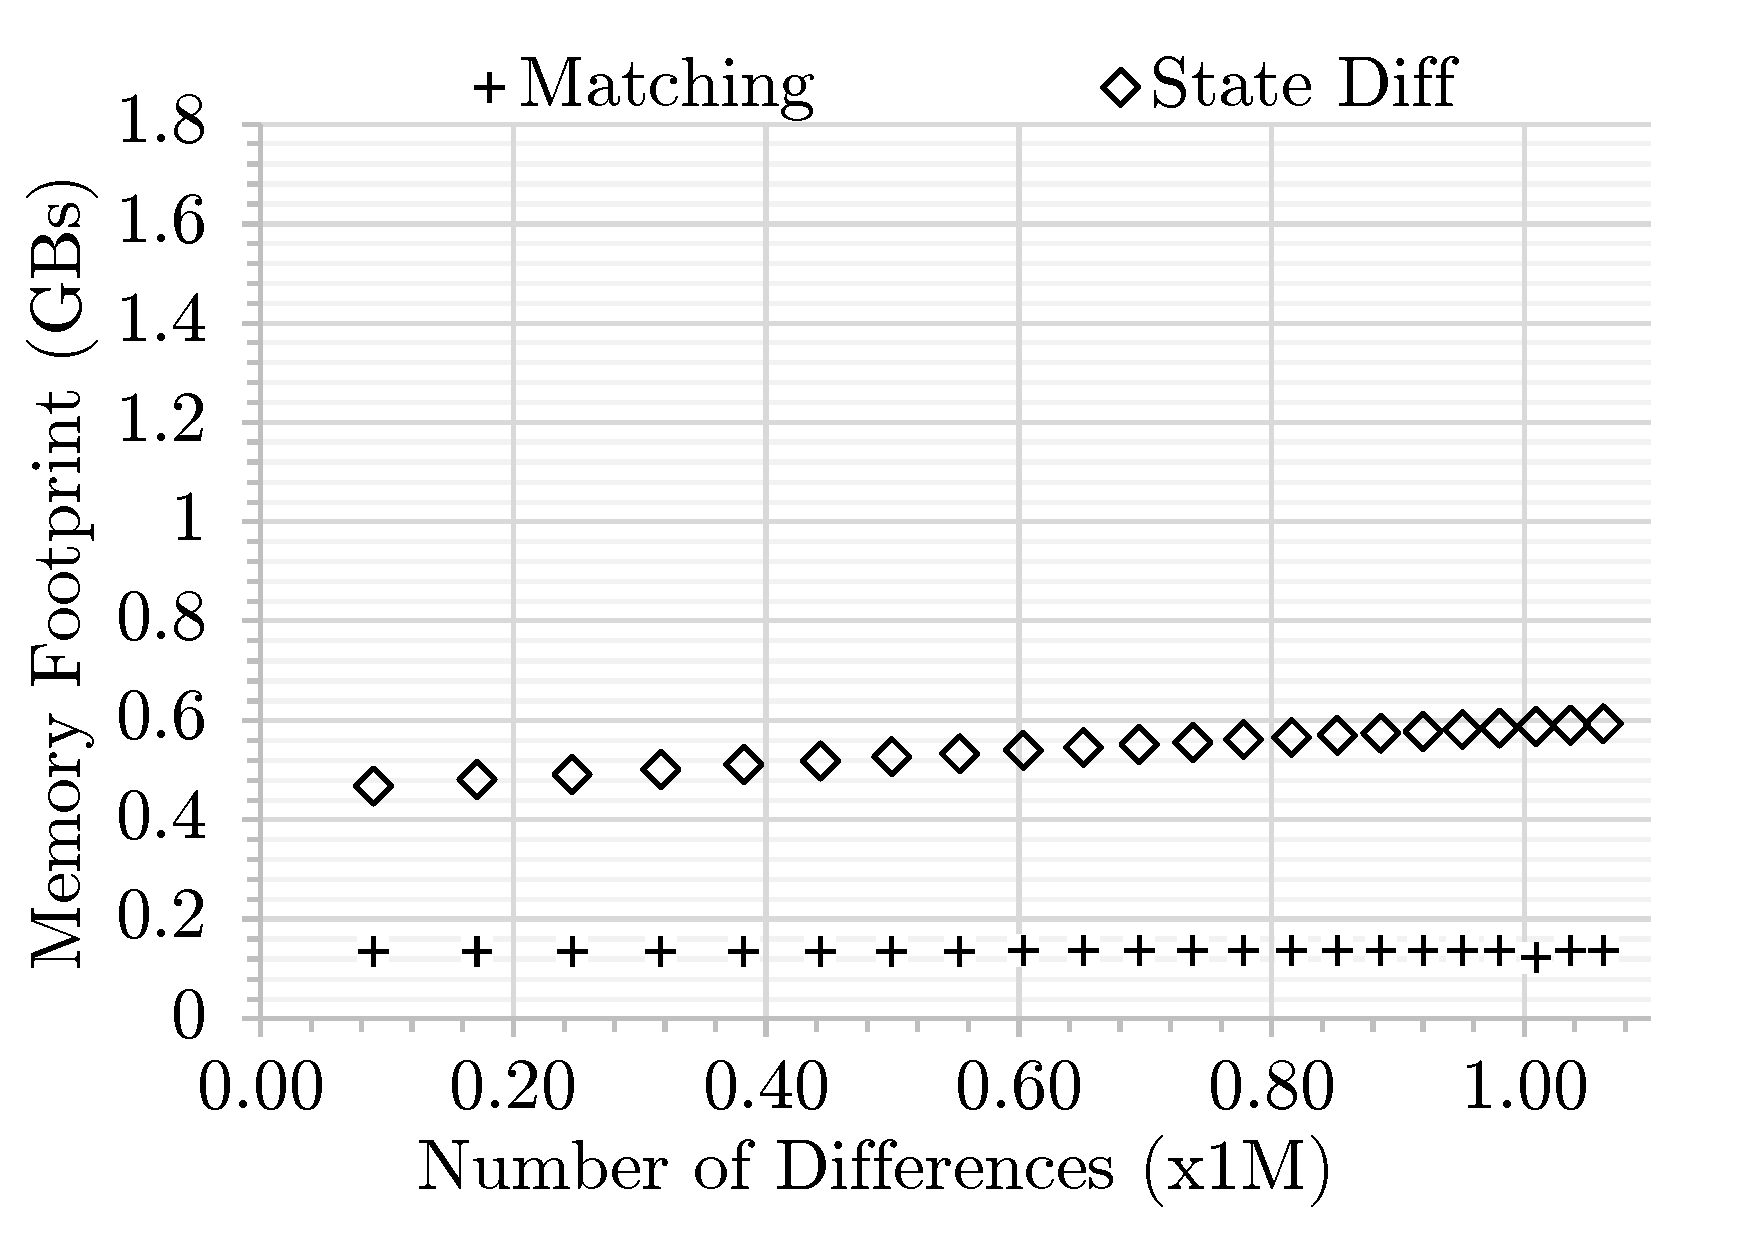
\includegraphics[width=\linewidth]{Memory-StateDiff-Detail}
        \caption{state-based memory footprint}
        \label{fig:memory_statediff_detail}
    \end{subfigure}
    \caption{Breakdown view of execution time and memory in Figure \ref{fig:change_vs_state}.}
    \label{fig:time_memory_detail}
\end{figure}

For the state-based comparison in Fig. \ref{fig:time_statediff_detail}, the comparison time only experiences a slight increase as the number of identified differences inclines. This slight increase is contributed mainly by the state-based diffing time while matching time tends to only contribute constantly due to the very small changes of the total elements (Figures \ref{fig:modification_course}, \ref{fig:model_size}).

Nevertheless, the change-based comparison also comes with a drawback on memory footprint since it consumes more space than the state-based comparison does (see Figure \ref{fig:memory_diffs}). Fig. \ref{fig:memory_changediff_detail} breaks down the memory footprint of the change-based comparison into three factors: the loaded change events, element tree, and diffs. As the number of differences grows, a great deal of events is generated. These events have to be loaded into memory since the information that they contain are important for the construction of the element tree. The memory used for these events grows exponentially against the number of differences since as the events increase some of these events do not contribute to the addition of new differences their memory space still needs to be retained. In our evaluation, the element tree occupies most of the memory footprint since it mimics the partial states -- elements and features -- of the models that are affected by the changes. In our technical implementation, a feature can have many instances -- one instance for each element (As a comparison, in the EMF implementation, there is only one instance for a feature. The feature is used as a key so that different elements can have the same feature that maps to different values simultaneously). This contributes to the large memory footprint used by the element three. The identified change-based diffs, the third factor, are the smallest factor that contributes to the memory footprint of the change-based comparison. 

For the state-based comparison in Fig. \ref{fig:memory_statediff_detail}, the memory footprint only inclines slightly along the increase of differences. A large part of the memory footprint is used to represent the identified differences, while the memory used for matches tends to be constant as the changes of the total elements are very small -- less new elements means less memory needs to be allocated for new matches (Figures \ref{fig:modification_course}, \ref{fig:model_size}). 

Based on the findings, we argue that the change-based comparison approach works at its best for large models that have been modified in a moderate number of changes. Models that have been excessively modified could impair the performance of change-based comparison as a great deal of change records have to be read and loaded into memory. 

\subsection{Limitation and Threat to Validity}
\label{sec:limitation_and_Threat_to_validity}
The proposed change-based comparison comes with a limitation that it heavily relies on the use of identifiers to efficiently address modified elements. Applying change-based persistent to models that use URI fragments as element's identifiers face a challenge that an element's identifier is always changing when it is moved to another location in a model. The evaluation of the proposed change-based comparison is limited to the Java metamodel only. Thus, there is no guarantee it will always work on models with different metamodels. Although, we have tried to cover as much as common changes made in EMF models (e.g. performing \textit{add}/\textit{remove}/\textit{set}/\textit{move} operations on \textit{single}/\textit{multi}-\textit{valued} features, \textit{attribute}/\textit{reference} features, or \textit{containment}/\textit{non}-\textit{containment} references), the random modification made in the evaluation does not largely reflect the evolution of models in the real world. This is challenging as different domains can have their own patterns of model evolution -- different problems, metamodels, modellers, etc.

\section{Related Work}
\label{sec:related_work}
There are existing tools for model comparison. SiDiff \cite{Treude2007SiDiff} and DSMDiff \cite{lin2009dsmdiff} view models as graphs. They create matches and define differences between elements based on the similarity of their features. However, both are limited in flexibility to exploit the metamodel or particularities of a modelling language. EMF Compare \cite{emfcompare2018developer}, an established tool for model comparison and merging, addresses this by providing an extensible platform which users can define custom algorithms for matching, diffing, conflict detection, and merging. Flexibility is also offered by ECL (Epsilon Comparison Language) \cite{kolovos2009ecl}, a hybrid, rule-based language for model comparison, which allows users to specify algorithms to match elements of homogeneous/heterogeneous models. All these tools work at the structural level; they compare models based on the states of models.

AMOR \cite{DBLP:conf/sfm/BroschKLSWW12}, a model versioning platform, also compares models in state-based. However, it also uses records of changes/operations of models to improve the precision of conflict detection and resolution. For example, multiple conflicts caused by a composite operation should be resolved as one package, not as an individual conflict, to ensure consistency of resolution. EMFStore \cite{koegel2010emfstore} is a version control system for EMF models that stores model versions as packages of operations. Since it works purely in operations without considering the states of models, every operation is treated as a new change. Thus, concurrent operations that change the same feature to the same value are treated as conflicting operations. Moreover, owning its version control system prevents users to use common textual version control systems (e.g. Git, SVN) for their models.  

%We differentiate our approach in that it compares two models by exploiting information available in their change records to identify differences in their states. Models are still persisted in change-based format. However, to speed up model comparison, our approach constructs only partial states of the models, thus reducing the scope of comparison only to elements affected by recent changes since the last version.   

\section{Conclusions and Future Work}
\label{sec:conclusion_and_future_work}
In this paper, we have proposed our approach to optimising model comparison by exploiting the information contained in change-based persistence to localise comparison only to elements affected by recent changes. Our change-based persistence contains information that is enough to reconstruct an element tree -- a mapping of affected elements and features of models being compared. By iterating through elements and features in the element tree and comparing their properties, we can define their differences. Using such approach, we can produce model comparison that is faster than traditional, state-based model comparison as shown in our evaluation. However, this approach also comes with a cost on memory footprint as it needs to load change events from a change-based persistence into main memory in order to operate. The next challenge for future work is to identify strategies to merge models optimally and persist the merging in the change-based way. 

\backmatter

\emph{NB: Please be sure to include DOIs (Digital Object Identifiers) for all cited articles, where available}

\bibliographystyle{alphaurl}
\bibliography{references}

\abouttheauthors

\begin{acknowledgments}
This work was partly supported by through a scholarship managed by \emph{Lembaga Pengelola Dana Pendidikan Indonesia} (Indonesia Endowment Fund for Education).
\end{acknowledgments}

\end{document}
